% Customizable fields and text areas start with % >> below.
% Lines starting with the comment character (%) are normally removed before release outside the collaboration, but not those comments ending lines

% svn info. These are modified by svn at checkout time.
% The last version of these macros found before the maketitle will be the one on the front page,
% so only the main file is tracked.
% Do not edit by hand!
\RCS$Revision: 57905 $
\RCS$HeadURL: svn+ssh://pivarski@svn.cern.ch/reps/tdr2/notes/AN-11-180/trunk/AN-11-180.tex $
\RCS$Id: AN-11-180.tex 57905 2011-05-27 08:42:28Z alschmid $
%%%%%%%%%%%%% ptdr definitions %%%%%%%%%%%%%%%%%%%%%
%%%%%%%%%%%%%%%%%%%%%%%%%%%%%%%%%%%%%%%%%%%%%%%%%%%%%%%%%%%%%%%%%%%%%
%
%  Common definitions
%
%  N.B. use of \providecommand rather than \newcommand means
%       that a definition is ignored if already specified
%
%                                              L. Taylor 18 Feb 2005
%%%%%%%%%%%%%%%%%%%%%%%%%%%%%%%%%%%%%%%%%%%%%%%%%%%%%%%%%%%%%%%%%%%%

% Some shorthand
% turn off italics
\newcommand {\etal}{\mbox{et al.}\xspace} %et al. - no preceding comma
\newcommand {\ie}{\mbox{i.e.}\xspace}     %i.e.
\newcommand {\eg}{\mbox{e.g.}\xspace}     %e.g.
\newcommand {\etc}{\mbox{etc.}\xspace}     %etc.
\newcommand {\vs}{\mbox{\sl vs.}\xspace}      %vs.
\newcommand {\mdash}{\ensuremath{\mathrm{-}}} % for use within formulas

% some terms whose definition we may change
\newcommand {\Lone}{Level-1\xspace} % Level-1 or L1 ?
\newcommand {\Ltwo}{Level-2\xspace}
\newcommand {\Lthree}{Level-3\xspace}

% Some software programs (alphabetized)
\providecommand{\ACERMC} {\textsc{AcerMC}\xspace}
\providecommand{\ALPGEN} {{\textsc{alpgen}}\xspace}
\providecommand{\CHARYBDIS} {{\textsc{charybdis}}\xspace}
\providecommand{\CMKIN} {\textsc{cmkin}\xspace}
\providecommand{\CMSIM} {{\textsc{cmsim}}\xspace}
\providecommand{\CMSSW} {{\textsc{cmssw}}\xspace}
\providecommand{\COBRA} {{\textsc{cobra}}\xspace}
\providecommand{\COCOA} {{\textsc{cocoa}}\xspace}
\providecommand{\COMPHEP} {\textsc{CompHEP}\xspace}
\providecommand{\EVTGEN} {{\textsc{evtgen}}\xspace}
\providecommand{\FAMOS} {{\textsc{famos}}\xspace}
\providecommand{\GARCON} {\textsc{garcon}\xspace}
\providecommand{\GARFIELD} {{\textsc{garfield}}\xspace}
\providecommand{\GEANE} {{\textsc{geane}}\xspace}
\providecommand{\GEANTfour} {{\textsc{geant4}}\xspace}
\providecommand{\GEANTthree} {{\textsc{geant3}}\xspace}
\providecommand{\GEANT} {{\textsc{geant}}\xspace}
\providecommand{\HDECAY} {\textsc{hdecay}\xspace}
\providecommand{\HERWIG} {{\textsc{herwig}}\xspace}
\providecommand{\HIGLU} {{\textsc{higlu}}\xspace}
\providecommand{\HIJING} {{\textsc{hijing}}\xspace}
\providecommand{\IGUANA} {\textsc{iguana}\xspace}
\providecommand{\ISAJET} {{\textsc{isajet}}\xspace}
\providecommand{\ISAPYTHIA} {{\textsc{isapythia}}\xspace}
\providecommand{\ISASUGRA} {{\textsc{isasugra}}\xspace}
\providecommand{\ISASUSY} {{\textsc{isasusy}}\xspace}
\providecommand{\ISAWIG} {{\textsc{isawig}}\xspace}
\providecommand{\MADGRAPH} {\textsc{MadGraph}\xspace}
\providecommand{\MCATNLO} {\textsc{mc@nlo}\xspace}
\providecommand{\MCFM} {\textsc{mcfm}\xspace}
\providecommand{\MILLEPEDE} {{\textsc{millepede}}\xspace}
\providecommand{\ORCA} {{\textsc{orca}}\xspace}
\providecommand{\OSCAR} {{\textsc{oscar}}\xspace}
\providecommand{\PHOTOS} {\textsc{photos}\xspace}
\providecommand{\PROSPINO} {\textsc{prospino}\xspace}
\providecommand{\PYTHIA} {{\textsc{pythia}}\xspace}
\providecommand{\SHERPA} {{\textsc{sherpa}}\xspace}
\providecommand{\TAUOLA} {\textsc{tauola}\xspace}
\providecommand{\TOPREX} {\textsc{TopReX}\xspace}
\providecommand{\XDAQ} {{\textsc{xdaq}}\xspace}


%  Experiments
\newcommand {\DZERO}{D\O\xspace}     %etc.


% Measurements and units...

\newcommand{\de}{\ensuremath{^\circ}}
\newcommand{\ten}[1]{\ensuremath{\times \text{10}^\text{#1}}}
\newcommand{\unit}[1]{\ensuremath{\text{\,#1}}\xspace}
\newcommand{\mum}{\ensuremath{\,\mu\text{m}}\xspace}
\newcommand{\micron}{\ensuremath{\,\mu\text{m}}\xspace}
\newcommand{\cm}{\ensuremath{\,\text{cm}}\xspace}
\newcommand{\mm}{\ensuremath{\,\text{mm}}\xspace}
\newcommand{\mus}{\ensuremath{\,\mu\text{s}}\xspace}
\newcommand{\keV}{\ensuremath{\,\text{ke\hspace{-.08em}V}}\xspace}
\newcommand{\MeV}{\ensuremath{\,\text{Me\hspace{-.08em}V}}\xspace}
\newcommand{\GeV}{\ensuremath{\,\text{Ge\hspace{-.08em}V}}\xspace}
\newcommand{\TeV}{\ensuremath{\,\text{Te\hspace{-.08em}V}}\xspace}
\newcommand{\PeV}{\ensuremath{\,\text{Pe\hspace{-.08em}V}}\xspace}
\newcommand{\keVc}{\ensuremath{{\,\text{ke\hspace{-.08em}V\hspace{-0.16em}/\hspace{-0.08em}}c}}\xspace}
\newcommand{\MeVc}{\ensuremath{{\,\text{Me\hspace{-.08em}V\hspace{-0.16em}/\hspace{-0.08em}}c}}\xspace}
\newcommand{\GeVc}{\ensuremath{{\,\text{Ge\hspace{-.08em}V\hspace{-0.16em}/\hspace{-0.08em}}c}}\xspace}
\newcommand{\TeVc}{\ensuremath{{\,\text{Te\hspace{-.08em}V\hspace{-0.16em}/\hspace{-0.08em}}c}}\xspace}
\newcommand{\keVcc}{\ensuremath{{\,\text{ke\hspace{-.08em}V\hspace{-0.16em}/\hspace{-0.08em}}c^\text{2}}}\xspace}
\newcommand{\MeVcc}{\ensuremath{{\,\text{Me\hspace{-.08em}V\hspace{-0.16em}/\hspace{-0.08em}}c^\text{2}}}\xspace}
\newcommand{\GeVcc}{\ensuremath{{\,\text{Ge\hspace{-.08em}V\hspace{-0.16em}/\hspace{-0.08em}}c^\text{2}}}\xspace}
\newcommand{\TeVcc}{\ensuremath{{\,\text{Te\hspace{-.08em}V\hspace{-0.16em}/\hspace{-0.08em}}c^\text{2}}}\xspace}

\newcommand{\pbinv} {\mbox{\ensuremath{\,\text{pb}^\text{$-$1}}}\xspace}
\newcommand{\fbinv} {\mbox{\ensuremath{\,\text{fb}^\text{$-$1}}}\xspace}
\newcommand{\nbinv} {\mbox{\ensuremath{\,\text{nb}^\text{$-$1}}}\xspace}
\newcommand{\percms}{\ensuremath{\,\text{cm}^\text{$-$2}\,\text{s}^\text{$-$1}}\xspace}
\newcommand{\lumi}{\ensuremath{\mathcal{L}}\xspace}
\newcommand{\Lumi}{\ensuremath{\mathcal{L}}\xspace}%both upper and lower
%
% Need a convention here:
\newcommand{\LvLow}  {\ensuremath{\mathcal{L}=\text{10}^\text{32}\,\text{cm}^\text{$-$2}\,\text{s}^\text{$-$1}}\xspace}
\newcommand{\LLow}   {\ensuremath{\mathcal{L}=\text{10}^\text{33}\,\text{cm}^\text{$-$2}\,\text{s}^\text{$-$1}}\xspace}
\newcommand{\lowlumi}{\ensuremath{\mathcal{L}=\text{2}\times \text{10}^\text{33}\,\text{cm}^\text{$-$2}\,\text{s}^\text{$-$1}}\xspace}
\newcommand{\LMed}   {\ensuremath{\mathcal{L}=\text{2}\times \text{10}^\text{33}\,\text{cm}^\text{$-$2}\,\text{s}^\text{$-$1}}\xspace}
\newcommand{\LHigh}  {\ensuremath{\mathcal{L}=\text{10}^\text{34}\,\text{cm}^\text{-2}\,\text{s}^\text{$-$1}}\xspace}
\newcommand{\hilumi} {\ensuremath{\mathcal{L}=\text{10}^\text{34}\,\text{cm}^\text{-2}\,\text{s}^\text{$-$1}}\xspace}

% Some usual physics terms

\newcommand{\zp}{\ensuremath{\mathrm{Z}^\prime}\xspace}

% SM (still to be classified)

\newcommand{\kt}{\ensuremath{k_{\mathrm{T}}}\xspace}
\newcommand{\BC}{\ensuremath{{B_{\mathrm{c}}}}\xspace}
\newcommand{\bbarc}{\ensuremath{{\overline{b}c}}\xspace}
\newcommand{\bbbar}{\ensuremath{{b\overline{b}}}\xspace}
\newcommand{\ccbar}{\ensuremath{{c\overline{c}}}\xspace}
\newcommand{\JPsi}{\ensuremath{{J}\hspace{-.08em}/\hspace{-.14em}\psi}\xspace}
\newcommand{\bspsiphi}{\ensuremath{B_s \to \JPsi\, \phi}\xspace}
%\newcommand{\ttbar}{\ensuremath{{t\overline{t}}}\xspace}
\newcommand{\AFB}{\ensuremath{A_\text{FB}}\xspace}
\newcommand{\EE}{\ensuremath{e^+e^-}\xspace}
\newcommand{\MM}{\ensuremath{\mu^+\mu^-}\xspace}
\newcommand{\TT}{\ensuremath{\tau^+\tau^-}\xspace}
\newcommand{\wangle}{\ensuremath{\sin^{2}\theta_{\text{eff}}^\text{lept}(M^2_\mathrm{Z})}\xspace}
\newcommand{\ttbar}{\ensuremath{{t\overline{t}}}\xspace}
\newcommand{\stat}{\ensuremath{\,\text{(stat.)}}\xspace}
\newcommand{\syst}{\ensuremath{\,\text{(syst.)}}\xspace}
% these moved to similar defs
%\newcommand{\Etmiss}{\ensuremath{E_{\mathrm{T}\!{\rm miss}}}}
%\newcommand{\VEtmiss}{\ensuremath{{\vec E}_{\mathrm{T}\!{\rm miss}}}}

%%%  E-gamma definitions
\newcommand{\HGG}{\ensuremath{\mathrm{H}\to\gamma\gamma}}
\newcommand{\gev}{\GeV}
\newcommand{\GAMJET}{\ensuremath{\gamma + \text{jet}}}
\newcommand{\PPTOJETS}{\ensuremath{\mathrm{pp}\to\text{jets}}}
\newcommand{\PPTOGG}{\ensuremath{\mathrm{pp}\to\gamma\gamma}}
\newcommand{\PPTOGAMJET}{\ensuremath{\mathrm{pp}\to\gamma +
\mathrm{jet}
}}
\newcommand{\MH}{\ensuremath{\mathrm{M_{\mathrm{H}}}}}
\newcommand{\RNINE}{\ensuremath{\mathrm{R}_\mathrm{9}}}
\newcommand{\DR}{\ensuremath{\Delta\mathrm{R}}}



% Physics symbols ...

\newcommand{\PT}{\ensuremath{p_{\mathrm{T}}}\xspace}
\newcommand{\pt}{\ensuremath{p_{\mathrm{T}}}\xspace}
\newcommand{\ET}{\ensuremath{E_{\mathrm{T}}}\xspace}
\newcommand{\HT}{\ensuremath{H_{\mathrm{T}}}\xspace}
\newcommand{\et}{\ensuremath{E_{\mathrm{T}}}\xspace}
\newcommand{\Em}{\ensuremath{E\!\!\!/}\xspace}
\newcommand{\Pm}{\ensuremath{p\!\!\!/}\xspace}
\newcommand{\PTm}{\ensuremath{{p\!\!\!/}_{\mathrm{T}}}\xspace}
\newcommand{\ETm}{\ensuremath{E_{\mathrm{T}}^{\text{miss}}}\xspace}
\newcommand{\MET}{\ensuremath{E_{\mathrm{T}}^{\text{miss}}}\xspace}
\newcommand{\ETmiss}{\ensuremath{E_{\mathrm{T}}^{\text{miss}}}\xspace}
\newcommand{\VEtmiss}{\ensuremath{{\vec E}_{\mathrm{T}}^{\text{miss}}}\xspace}

%%%%%%
% From Albert
%

\newcommand{\ga}{\ensuremath{\gtrsim}}
\newcommand{\la}{\ensuremath{\lesssim}}
%\def\ga{\mathrel{\rlap{\raise.6ex\hbox{$>$}}{\lower.6ex\hbox{$\sim$}}}}
%\def\la{\mathrel{\rlap{\raise.6ex\hbox{$<$}}{\lower.6ex\hbox{$\sim$}}}}
%
\newcommand{\swsq}{\ensuremath{\sin^2\theta_W}\xspace}
\newcommand{\cwsq}{\ensuremath{\cos^2\theta_W}\xspace}
\newcommand{\tanb}{\ensuremath{\tan\beta}\xspace}
\newcommand{\tanbsq}{\ensuremath{\tan^{2}\beta}\xspace}
\newcommand{\sidb}{\ensuremath{\sin 2\beta}\xspace}
\newcommand{\alpS}{\ensuremath{\alpha_S}\xspace}
\newcommand{\alpt}{\ensuremath{\tilde{\alpha}}\xspace}

\newcommand{\QL}{\ensuremath{Q_L}\xspace}
\newcommand{\sQ}{\ensuremath{\tilde{Q}}\xspace}
\newcommand{\sQL}{\ensuremath{\tilde{Q}_L}\xspace}
\newcommand{\ULC}{\ensuremath{U_L^C}\xspace}
\newcommand{\sUC}{\ensuremath{\tilde{U}^C}\xspace}
\newcommand{\sULC}{\ensuremath{\tilde{U}_L^C}\xspace}
\newcommand{\DLC}{\ensuremath{D_L^C}\xspace}
\newcommand{\sDC}{\ensuremath{\tilde{D}^C}\xspace}
\newcommand{\sDLC}{\ensuremath{\tilde{D}_L^C}\xspace}
\newcommand{\LL}{\ensuremath{L_L}\xspace}
\newcommand{\sL}{\ensuremath{\tilde{L}}\xspace}
\newcommand{\sLL}{\ensuremath{\tilde{L}_L}\xspace}
\newcommand{\ELC}{\ensuremath{E_L^C}\xspace}
\newcommand{\sEC}{\ensuremath{\tilde{E}^C}\xspace}
\newcommand{\sELC}{\ensuremath{\tilde{E}_L^C}\xspace}
\newcommand{\sEL}{\ensuremath{\tilde{E}_L}\xspace}
\newcommand{\sER}{\ensuremath{\tilde{E}_R}\xspace}
\newcommand{\sFer}{\ensuremath{\tilde{f}}\xspace}
\newcommand{\sQua}{\ensuremath{\tilde{q}}\xspace}
\newcommand{\sUp}{\ensuremath{\tilde{u}}\xspace}
\newcommand{\suL}{\ensuremath{\tilde{u}_L}\xspace}
\newcommand{\suR}{\ensuremath{\tilde{u}_R}\xspace}
\newcommand{\sDw}{\ensuremath{\tilde{d}}\xspace}
\newcommand{\sdL}{\ensuremath{\tilde{d}_L}\xspace}
\newcommand{\sdR}{\ensuremath{\tilde{d}_R}\xspace}
\newcommand{\sTop}{\ensuremath{\tilde{t}}\xspace}
\newcommand{\stL}{\ensuremath{\tilde{t}_L}\xspace}
\newcommand{\stR}{\ensuremath{\tilde{t}_R}\xspace}
\newcommand{\stone}{\ensuremath{\tilde{t}_1}\xspace}
\newcommand{\sttwo}{\ensuremath{\tilde{t}_2}\xspace}
\newcommand{\sBot}{\ensuremath{\tilde{b}}\xspace}
\newcommand{\sbL}{\ensuremath{\tilde{b}_L}\xspace}
\newcommand{\sbR}{\ensuremath{\tilde{b}_R}\xspace}
\newcommand{\sbone}{\ensuremath{\tilde{b}_1}\xspace}
\newcommand{\sbtwo}{\ensuremath{\tilde{b}_2}\xspace}
\newcommand{\sLep}{\ensuremath{\tilde{l}}\xspace}
\newcommand{\sLepC}{\ensuremath{\tilde{l}^C}\xspace}
\newcommand{\sEl}{\ensuremath{\tilde{e}}\xspace}
\newcommand{\sElC}{\ensuremath{\tilde{e}^C}\xspace}
\newcommand{\seL}{\ensuremath{\tilde{e}_L}\xspace}
\newcommand{\seR}{\ensuremath{\tilde{e}_R}\xspace}
\newcommand{\snL}{\ensuremath{\tilde{\nu}_L}\xspace}
\newcommand{\sMu}{\ensuremath{\tilde{\mu}}\xspace}
\newcommand{\sNu}{\ensuremath{\tilde{\nu}}\xspace}
\newcommand{\sTau}{\ensuremath{\tilde{\tau}}\xspace}
\newcommand{\Glu}{\ensuremath{g}\xspace}
\newcommand{\sGlu}{\ensuremath{\tilde{g}}\xspace}
\newcommand{\Wpm}{\ensuremath{W^{\pm}}\xspace}
\newcommand{\sWpm}{\ensuremath{\tilde{W}^{\pm}}\xspace}
\newcommand{\Wz}{\ensuremath{W^{0}}\xspace}
\newcommand{\sWz}{\ensuremath{\tilde{W}^{0}}\xspace}
\newcommand{\sWino}{\ensuremath{\tilde{W}}\xspace}
\newcommand{\Bz}{\ensuremath{B^{0}}\xspace}
\newcommand{\sBz}{\ensuremath{\tilde{B}^{0}}\xspace}
\newcommand{\sBino}{\ensuremath{\tilde{B}}\xspace}
\newcommand{\Zz}{\ensuremath{Z^{0}}\xspace}
\newcommand{\sZino}{\ensuremath{\tilde{Z}^{0}}\xspace}
\newcommand{\sGam}{\ensuremath{\tilde{\gamma}}\xspace}
\newcommand{\chiz}{\ensuremath{\tilde{\chi}^{0}}\xspace}
\newcommand{\chip}{\ensuremath{\tilde{\chi}^{+}}\xspace}
\newcommand{\chim}{\ensuremath{\tilde{\chi}^{-}}\xspace}
\newcommand{\chipm}{\ensuremath{\tilde{\chi}^{\pm}}\xspace}
\newcommand{\Hone}{\ensuremath{H_{d}}\xspace}
\newcommand{\sHone}{\ensuremath{\tilde{H}_{d}}\xspace}
\newcommand{\Htwo}{\ensuremath{H_{u}}\xspace}
\newcommand{\sHtwo}{\ensuremath{\tilde{H}_{u}}\xspace}
\newcommand{\sHig}{\ensuremath{\tilde{H}}\xspace}
\newcommand{\sHa}{\ensuremath{\tilde{H}_{a}}\xspace}
\newcommand{\sHb}{\ensuremath{\tilde{H}_{b}}\xspace}
\newcommand{\sHpm}{\ensuremath{\tilde{H}^{\pm}}\xspace}
\newcommand{\hz}{\ensuremath{h^{0}}\xspace}
\newcommand{\Hz}{\ensuremath{H^{0}}\xspace}
\newcommand{\Az}{\ensuremath{A^{0}}\xspace}
\newcommand{\Hpm}{\ensuremath{H^{\pm}}\xspace}
\newcommand{\sGra}{\ensuremath{\tilde{G}}\xspace}
%
\newcommand{\mtil}{\ensuremath{\tilde{m}}\xspace}
%
\newcommand{\rpv}{\ensuremath{\rlap{\kern.2em/}R}\xspace}
\newcommand{\LLE}{\ensuremath{LL\bar{E}}\xspace}
\newcommand{\LQD}{\ensuremath{LQ\bar{D}}\xspace}
\newcommand{\UDD}{\ensuremath{\overline{UDD}}\xspace}
\newcommand{\Lam}{\ensuremath{\lambda}\xspace}
\newcommand{\Lamp}{\ensuremath{\lambda'}\xspace}
\newcommand{\Lampp}{\ensuremath{\lambda''}\xspace}
%
\newcommand{\spinbd}[2]{\ensuremath{\bar{#1}_{\dot{#2}}}\xspace}

\newcommand{\MD}{\ensuremath{{M_\mathrm{D}}}\xspace}% ED mass
\newcommand{\Mpl}{\ensuremath{{M_\mathrm{Pl}}}\xspace}% Planck mass
\newcommand{\Rinv} {\ensuremath{{R}^{-1}}\xspace}



%%%%%%%%%%%%%%%%%%%%%%%%%%%%%%%%%%%%%%%%%%%%%%%%%%%%%%%%%%%%%%%%%%%%
%
% Hyphenations (only need to add here if you get a nasty word break)
%
\hyphenation{en-viron-men-tal}%    just an example
 %These have been replaced by the equivalent style file
%%%%%%%%%%%%%%%  Title page %%%%%%%%%%%%%%%%%%%%%%%%
\cmsNoteHeader{AN-11-180} % This is over-written in the CMS environment: useful as preprint no. for export versions
% >> Title: please make sure that the non-TeX equivalent is in PDFTitle below
\title{Status of b-tagging tools for 2011 data analysis}

% >> Authors
%Author is always "The CMS Collaboration" for PAS and papers, so author, etc, below will be ignored in those cases
%For multiple affiliations, create an address entry for the combination
\address[neu]{University on the Moon}
\author[cern]{The CMS Collaboration}

% >> Date
% The date is in yyyy/mm/dd format. Today has been
% redefined to match, but if the date needs to be fixed, please write it in this fashion.
% For papers and PAS, \today is taken as the date the head file (this one) was last modified according to svn: see the RCS Id string above.
% For the final version it is best to "touch" the head file to make sure it has the latest date.
\date{\today}

% >> Abstract
% Abstract processing:
% 1. **DO NOT use \include or \input** to include the abstract: our abstract extractor will not search through other files than this one.
% 2. **DO NOT use %**                  to comment out sections of the abstract: the extractor will still grab those lines (and they won't be comments any longer!).
% 3. **DO NOT use tex macros**         in the abstract: External TeX parsers used on the abstract don't understand them.
\abstract{
The identification of jets containing the weak decay of a B-hadron is
an essential tool for a wide range of analyses in the context of the
Standard Model and beyond. A variety of algorithms exploit the long
lifetime and the presence of soft leptons to discriminate these jets
from those associated to light quarks. The status of the b-tagging
tools and their commissioning with 2011 data is presented. New
developments and improvements of the b-tagging algorithms are also
documented.  
}

% >> PDF Metadata
% Do not comment out the following hypersetup lines (metadata). They will disappear in NODRAFT mode and are needed by CDS.
% Also: make sure that the values of the metadata items are sensible. For APS submissions, they are automatically converted to APS keywords.
\hypersetup{%
pdfauthor={Alexander Schmidt},%
pdftitle={Status of b-tagging tools for 2011 data analysis},%
pdfsubject={CMS},%
pdfkeywords={CMS, BTV, physics, software}}

\maketitle %maketitle comes after all the front information has been supplied

% >> Text
%%%%%%%%%%%%%%%%%%%%%%%%%%%%%%%%  Begin text %%%%%%%%%%%%%%%%%%%%%%%%%%%%%
%% **DO NOT REMOVE THE BIBLIOGRAPHY** which is located before the appendix.
%% You can take the text between here and the bibiliography as an example which you should replace with the actual text of your document.
%% If you include other TeX files, be sure to use "\input{filename}" rather than "\input filename".
%% The latter works for you, but our parser looks for the braces and will break when uploading the document.
%%%%%%%%%%%%%%%
\section{Introduction}
The identification of jets originating from b quarks  is a crucial
element for many physics analyses. In particular, high branching ratios to b quarks characterize a variety
of Standard Model (SM) and discovery channels like the measurement of bottom or top pair
production, the search for Higgs bosons and different other New Physics scenarios. 

The hard fragmentation, the long lifetimes and high masses of B hadrons and the relatively
high fraction of semileptonic decays distinguish these jets from those originating from gluons,
light quarks and - to a lesser extent - from c quarks. Due to its precise inner tracking system
and its lepton identification capabilities the CMS experiment is particularly suited for exploiting
these features.

Detailed definitions of the studied quantities are given in
\cite{btaggingPAS2009}, along with an explanation of the b-tagging
algorithms. The b-tag commissioning  with first collision data at 7~TeV is reported in
\cite{btaggingPAS2010}. The present note presents an update of the
commissioning activities including data from the 2011 run. The
validation of the main variables is discussed in Sections \ref{sec:trackselection} to \ref{sec:muonjets}. One
of the main differences to \cite{btaggingPAS2010} is the presence of
pileup, which is discussed in Section \ref{sec:pileup}. The development and
commissioning of additional higher-level b-tagging algorithms is
documented in Section~\ref{sec:dvelopments}.  
\section{High Level Trigger}
responsible editor: Jyothsna\\
%add documentation about btag mu triggers and possibly some comments on the btag IP triggers used in PAGS.
Technical implementation to use b-tagging at High Level Trigger (HLT) enviromnent
exists since few years \textbf{FIX ME add 2006 and 2007 references here}.
These implementations exploit couple of properties of jets originating 
from b-quarks namely semi-leptonic decays and long lifetime. ``BTagMu'' 
implementation makes use of semi-leptonic b-decays and tags jets at
HLT containing muons associated to them. Lifetime based b-tagging
implementation referred to as ``BTagIP'' implementation relies mostly on 
offline equivalent of Track Counting High Efficiency algorithm for
tagging the jets at HLT. 

Implementation details of ``BTagMu'' and ``BTagIP'' along with the 
triggers developed for calibration and physics use cases is 
presented in the next sections.

\subsection{BTagMu HLT implementation and use cases}
Events containing a $\mu$ associated with a jet can be used to the
measure the b-tag performance from data. Since only paths using BTagMu
implementation are the b-tag calibration paths, these are
explicitly mentioned in the below description of the implementation.
The Level~1 seeds for these paths require a muon and a jet at Level~1
with $E_T$ cuts specific to each designed HLT path and are listed in 
Table \ref{btagmu}.

\begin{itemize}
\item Level-2: In 2011 Anti $k_T$ corrected calo jets are used as
  Level-2 jets. In order to reduce the HLT rates dijets are required
  at Level-2 with varying jet $E_T$ thresholds. These jet $E_T$ cuts
  are tuned to have enough statistics available offline to derive the
  efficiency and scale factors in various offline jet $E_T$ and $\eta$
  bins. In the recent data taking 20~GeV, 40~GeV, 70~GeV and 110~GeV
  are chosen as the thresholds.
\item Level-2.5: The soft lepton b-tagging algorithm is run on the 4 highest $E_T$ jets in the event
  with $E_T$ threshold chosen same as the $E_T$ cut on jets at
  Level-2. Level-2 muons, reconstructed using muon detector hits,
  are required to be near one of these 4 highest $E_T$ jets, $\Delta R(\mu, jet)
  ~<~0.4$, using the Soft Lepton b-tagging algorithm. Events pass if
  at least one jet is soft mu-tagged.
\item Level-3: Refined tracking is used to reconstruct Level-3
  muons. Only those Level-3 muons which pass $\mu~p_T~>5~GeV$ and have
  $>~0$ number of hits are used to select muon-in-jets with $\Delta R(\mu, jet)
  ~<~0.4$ requirement using the Soft Lepton b-tagging algorithm. Events pass if
  at least one jet is soft mu-tagged.
\end{itemize}

The Soft Lepton b-tagging algorithm used in both Level-2.5 and Level-3 make
use of the same methods used in the offline reconstruction and they
differ in muon and jet inputs at HLT wrt Offline.

The names of the ``BTagMu'' based triggers along with the Level-1
seeds are listed in Table \ref{btagmu}.

\begin{table}[htbp]
\begin{center}
\begin{tabular}{|c|c|c|c|}
\hline
\texfbf{Path name} & \textbf{Level-1 seed} & \textbf{HLT prescale} & \textbf{Rate @1E33}\\
\hline
HLT\_BTagMu\_DiJet20\_Mu5 & L1\_Mu3\_Jet16 & 350 & 1.62~Hz \\
HLT\_BTagMu\_DiJet40\_Mu5 & L1\_Mu3\_Jet20 & 100 & 1.32~Hz \\
HLT\_BTagMu\_DiJet70\_Mu5 & L1\_Mu3\_Jet28 & 15 & 1.36~Hz \\
HLT\_BTagMu\_DiJet110\_Mu5 & L1\_Mu3\_Jet28 & 2 & 1.62~Hz \\
\hline
\end{tabular}
\end{center}
\caption{}
\label{btagmu}
\end{table}

The offline selection required two jets of $\pt > 30\GeV$ and $|\eta|
< 2.4$ in order to stay within the tracker acceptance and in the
\pt\ range where b-tagging is typically applied. In order to increase 
the purity in ${\mathrm B} \to \mu + {\mathrm X}$ decays the event had 
to contain exactly one muon of $\pt > 6\GeV$ and $|\eta| < 2.4$ with
the following additional quality criteria:
\begin{itemize}
\item the muon was reconstructed as a ``GlobalMuon'' with at least one valid muon hit, more than one matching segment in the muon chambers and a $\chi^2/{\mathrm ndof}<10$;
\item the corresponding inner track had $>10$ hits with at least one hit in the pixel system and a $\chi^2/{\mathrm ndof}<10$;
\item the $z$-distance between the reference point of the muon and the selected primary vertex was $< 1$cm.
\end{itemize}
The muon had to be in a cone defined by $\DR < 0.4$ around the associated jet (``\muonjet'').

Turn on curves for the different BTagMu triggers have been computed by scaling the pT spectra for
the data collected by each trigger by its integrated luminosity, and dividing the so obtained
distribution by the one of the HLT\_BTagMu\_DiJet20\_Mu5 trigger. The turn on curve for
this last trigger has been computed by taking the pT spectrum of the muon-jetsin data collected
by the HLT\_Mu5 trigger as a reference. All these turn on curves are
shown in Fig. ~\ref{btagmuturnon}.

\begin{figure}[h!]
\centering
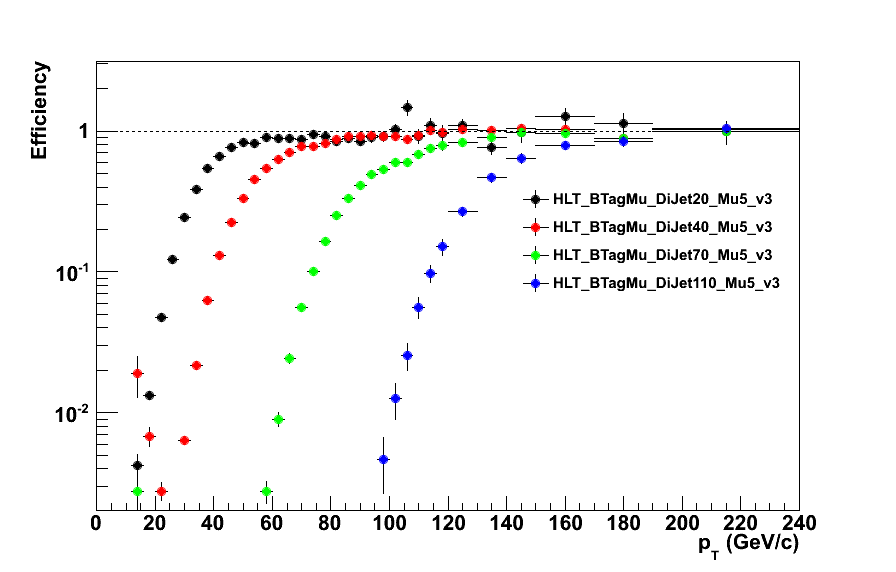
\includegraphics[width=0.65\textwidth]{figures/BTagMuTriggerTurnOn.png}
\caption{Turn on curve of all the above four paths using 2011 data}
\label{fig:btagmuturnon}
\end{figure}


\subsection{BTagIP HLT implementation and use cases}
Many standard model and exotic physics channels contain b jets in the
final state. By explicitly requiring b-tagged jets in the HLT paths 
for these physics channels, one can lower the jet $E_T$ thresholds 
than cutting harder on the jets for rate reduction, increasing the
purity as well as trigger efficiency for these channels.

A generic BTagIP implementation at HLT is described below. This
implementation is adapted to suit the needs of physics channels by the 
trigger developers. The Level-1 seeds are also up to the trigger
developers to choose depending on the physics channel and final state
they are interested in.

\begin{itemize}
\item Level-2: The jet $E_T$ thresholds and the number of jets vary
  depending on the needs of the physics channel.
\item Level-2.5: Tracks are reconstructed using the Pixel Tracker
  alone (each with at least 3 hits), and are then used to reconstruct
  the 1D primary vertex. The b-tag is run on 4-6 highest $E_T$ jets in
  the event with $E_T$ threshold chosen by the trigger developer,
  using the pixel tracks and the primary vertex as input. Most of the
  physics paths use Online Beam Spot in the transverse plane and fast
  estimation in Z as the primary vertex. 3D Primary vertex (PV) can also be
  used as reference. More details about the PV methods usage at HLT
  and the performnace are provide in the next subsection. Jets are
  tagged as b-jets if they have at least 1 or 2 tracks with 3D impact
  parameter significance greater than a threshold value tuned by the
  physics trigger developers. Events pass if at least one or two
  jets are b-tagged.
\item Level-3: Tracks are reconstructed regionally in a cone size
  $\Delta R~=~$ 0.25 either around the jets tagged as b-jets at
  Level-2.5 or around all the Level-2.5 jets. The choice of which jets
  are fed for the regional track reconstruction is also upto the
  developers. The track reconstruction is partial. stopping after 
  8 hits have been assigned to a track. The b-tag uses these tracks
  and the primary vertex reconstructed at Level-2.5. It selects jets
  having at least 2 tracks with 3D impact parameter significance
  greater than a threshold value tuned by the trigger
  developer. Events pass if at least one or two jets are b-tagged.
\end{itemize}

Trigger performance of couple of physics channels using BTagIP are
presented in Fig~\ref{QuadJetturnon} for QuadJet50\_BTagIP trigger path
and Fig~\ref{RA2bturnon} for HT300\_CentralJet30\_BTagIP\_PFMHT55
trigger path as a function of offline b-tag algorithms. 

QuadJet50\_BTagIP trigger path is developed for all hadronic ttbar
final state and to collect the events containing at least four jets at the HLT level with $E_T > 50$ GeV and
amongst at least one of them is required to be b-tagged by TCHE
algorithm at HLT. The cut TCHE cut chosen at HLT level is 2 for this
path and as can be seen in bottom plot in Fig~\ref{QuadJetturnon} the
efficiency is 50\% at offline TCHP value of 2.

SUSY analysis looking at missing $E_T$, jets and b-jet final state and
developed trigger path HT300\_CentralJet30\_BTagIP\_PFMHT55 to collect
such events. Jet with $E_T >$ 30 GeV is required to be b-tagged by
TCHE algorithm at HLT and the cut applied is at 4.

\begin{figure}[h!]
\centering
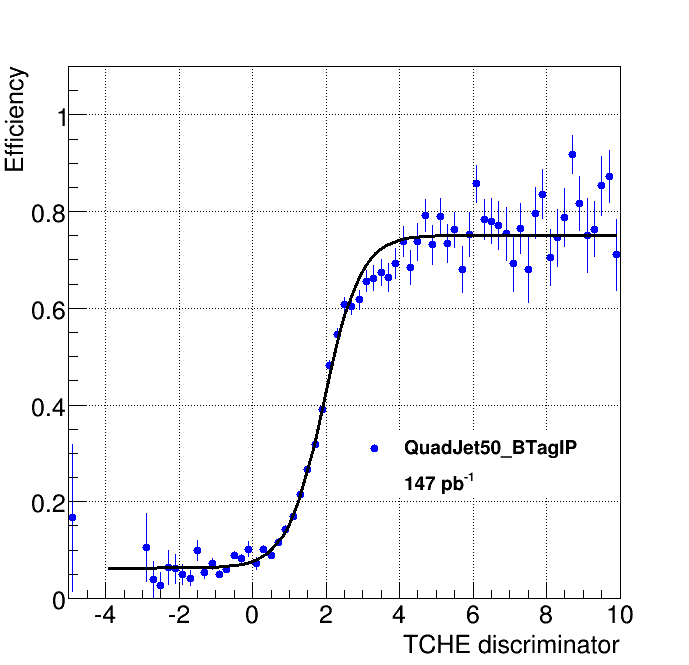
\includegraphics[width=0.5\textwidth]{figures/QuadBTagTCHE_turnOn.png}
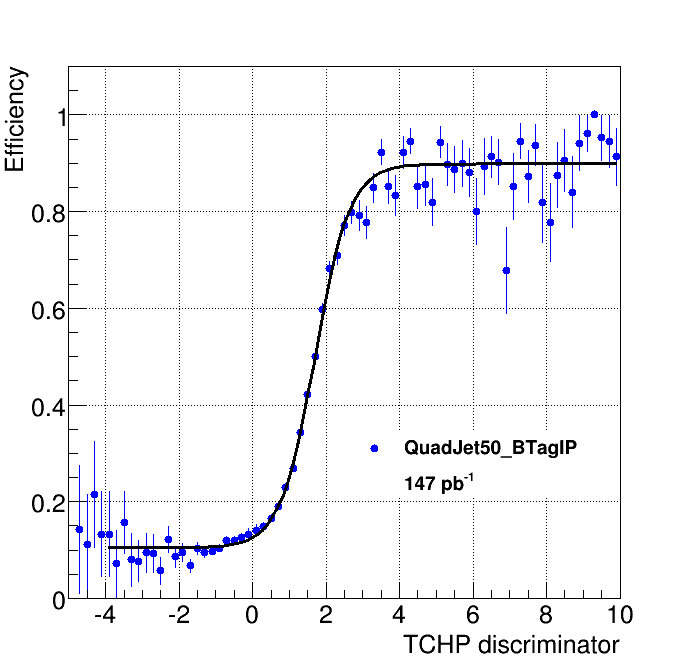
\includegraphics[width=0.5\textwidth]{figures/QuadBTagTCHP_turnOn.png}
\caption{Turn on curve for QuadJet50\_BTagIP trigger as a function of offline TCHE and TCHP
  discriminator obtained using 2011 data}
\label{fig:QuadJetturnon}
\end{figure}

\begin{figure}[h!]
\centering
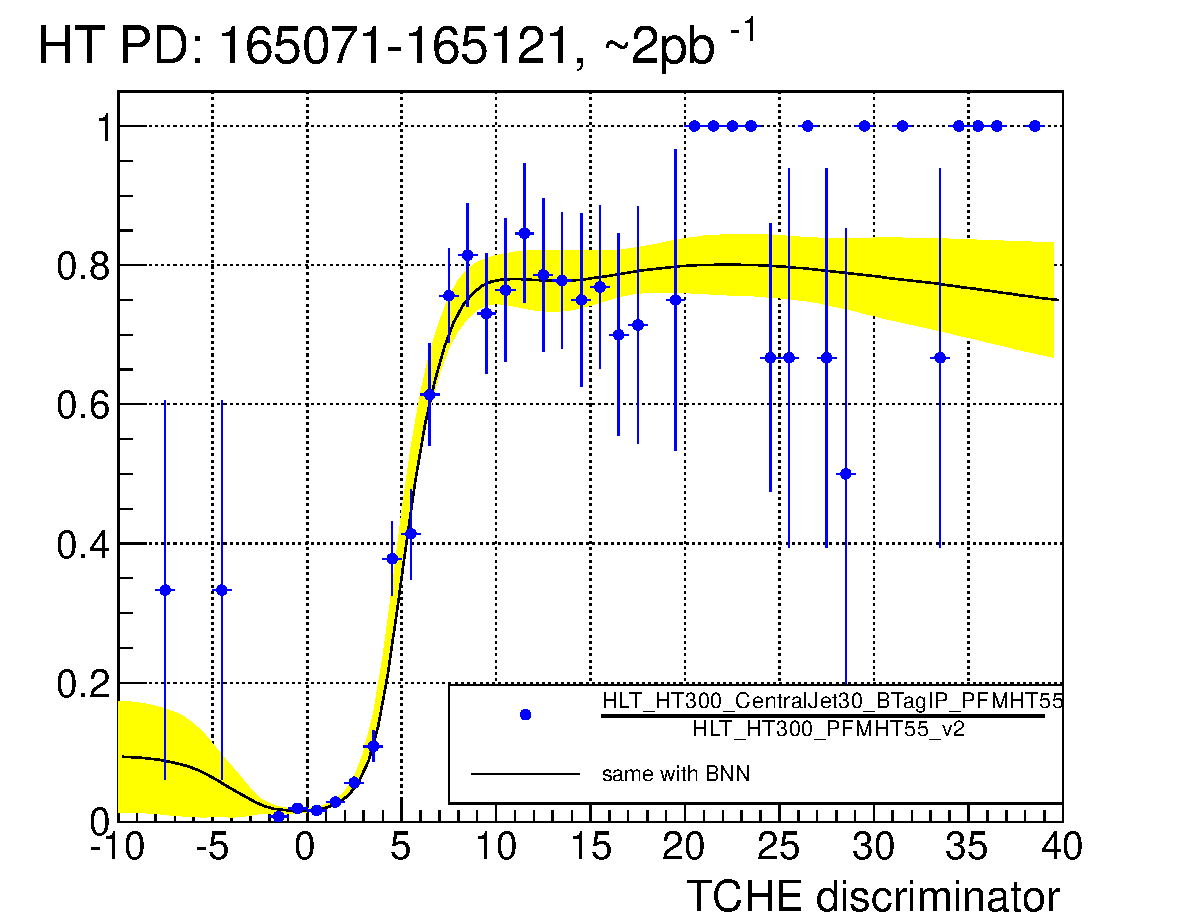
\includegraphics[width=0.5\textwidth]{figures/RA2bSUSY_TCHE_turnOn.pdf}
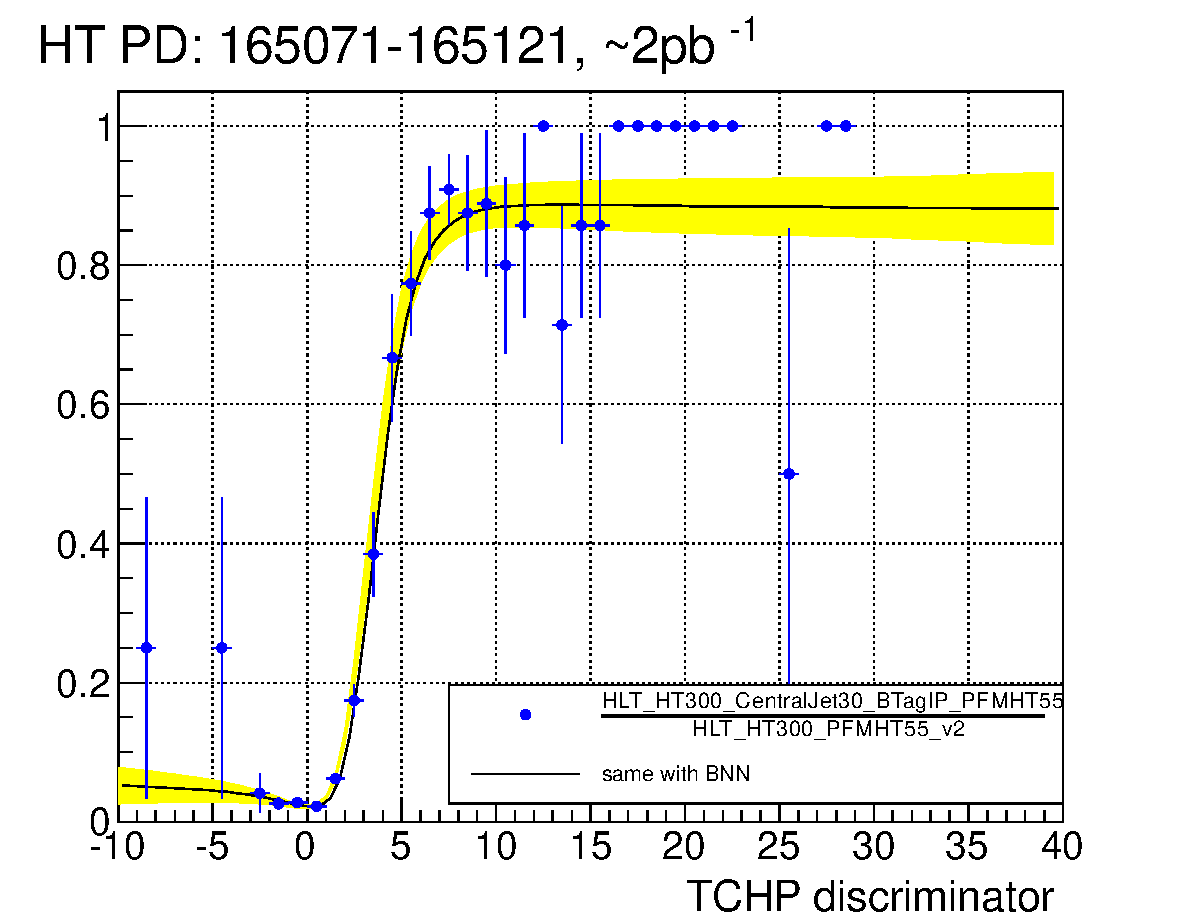
\includegraphics[width=0.5\textwidth]{figures/RA2bSUSY_TCHP_turnOn.pdf}
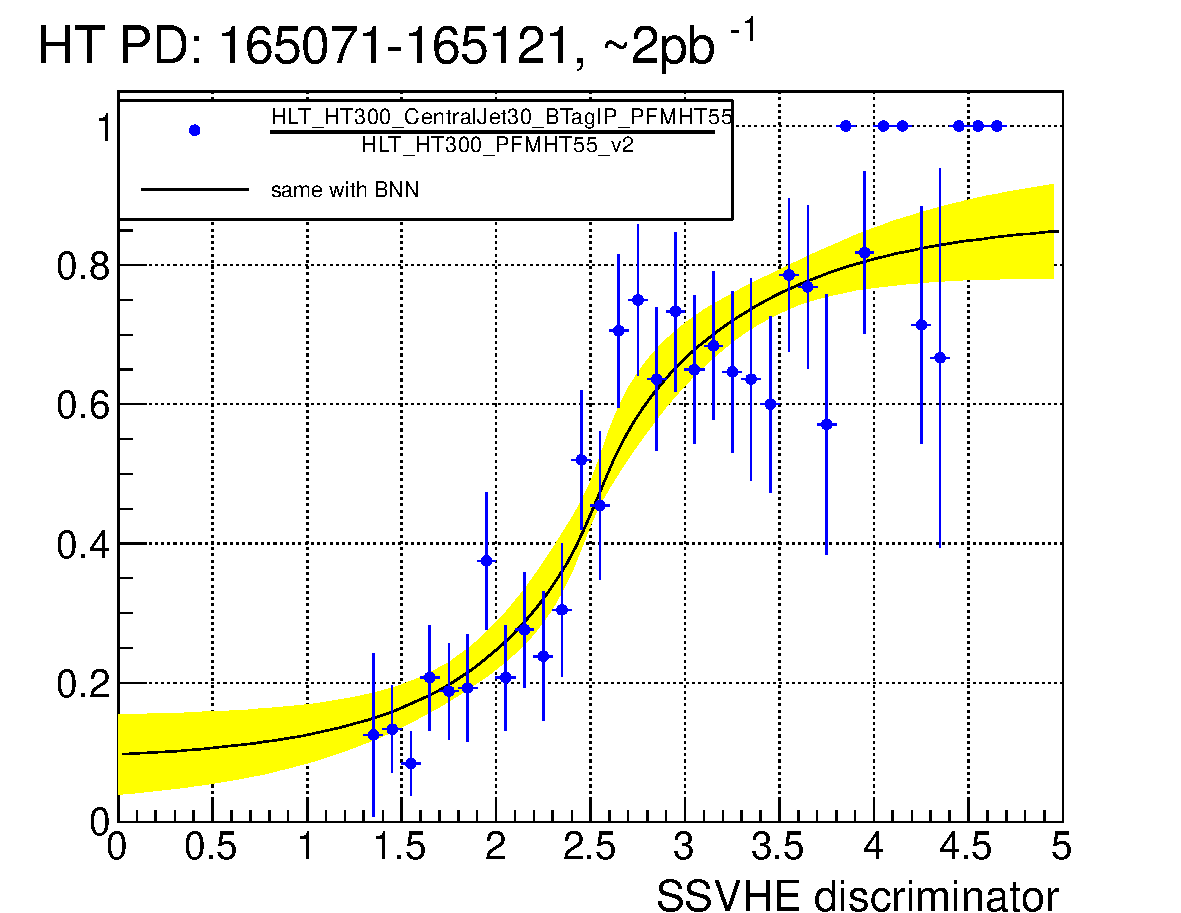
\includegraphics[width=0.5\textwidth]{figures/RA2bSUSY_SSVHE_turnOn.pdf}
\caption{Turn on curve for HT300\_CentralJet30\_BTagIP\_PFMHT55 as a
  function of offline TCHE, TCHP and SSVHE discriminator obtained using 2011 data}
\label{fig:RA2bturnon}
\end{figure}

\subsection{3D Primary Vertex}
responsible editor: Carlotta\\
To limit the CPU timing, the standard High Level Trigger reconstruction performs only a fast partial (1D) estimation of the primary vertex. Prompt pixel tracks are clustered in $z$ and the longitudinal vertex position is determined by the Divisive Vertex Fitter algorithm. The online beamspot is used as rough estimation of the transverse vertex coordinate.\\
%The pixel tracks in the event are clusterized into primary vertex candidates, and the vertex longitudinal position is determined by the Divisive Vertex Fitter as average of the $z$ of tracks in the cluster. A rough estimation of the transverse position is given by the beam spot. 
The full (3D) primary vertex reconstruction, implementing the Adaptive Vertex Fitter, could provide a reliable reference point for the track impact parameter calculation, input to the b-tagging algorithms, in case of movements of the beamspot. This will be crucial, at  high luminosity, for those trigger paths that rely on b-tagging to reduce the rate by a factor greater than 10. To avoid any bias from an incorrect beamspot position, no beam constraint is applied in the vertex fitting procedure.
%No beam constraint is applied, to exclude any bias in case the beamspot position is incorrect.
The Gap clusterizer is used.
To be included in the clusterization, pixel tracks are required to have at least 3 pixel hits, $\chi^{2}/ndof \leq$ 100.0, and transverse impact parameter significance $\leq$ 100.0.
An additional cut on the track momentum can be applied and tuned in order to achieve reasonably good performance with a limited CPU consumption. Tracks that pass the selection are grouped into primary vertex candidates if their $z$ distance to the nearest neighbor is smaller than 1 mm. A reconstructed primary vertex is finally rejected if the transverse distance to the beam is larger than 2 cm. 

The performance of the 3D primary vertex reconstruction, compared to the standard 1D, is evaluated using a Monte Carlo sample of QCD events with parton $p_{T}$ greater than 15 GeV$/c$, with on average 10 pile up events. 
Fig.\ref{efffake} and \ref{res} summarize the results for vertex finding efficiency, rate of fake vertices in the event, transverse and longitudinal position resolution, as a function of the $p_{T}$ cut applied to the pixel tracks.
% track and vertex sim-to-reco association?
%Fig.\ref{eff} shows the primary vertex finding efficiency provided by the 3D algorithm, as a function of the $p_{T}$ threshold applied to the pixel tracks. For the signal vertex, the efficiency is higher than 90\% up to a $p_{T}$ cut of 1.3 GeV$/c$, and is competitive with the performance of the 1D reconstruction, which applies a $p_{T} \geq$ 0.9 GeV selection. The rate of fake reconstructed vertices in the event, as a function of the $p_{T}$ threshold, is shown in Fig.\ref{faker}. For the standard 1D it is measured to be 12.5\%.
\begin{figure}
   \centering
   %%----start of first subfigure----
   \subfloat[]{
        \label{eff}           %% label for first subfigure
        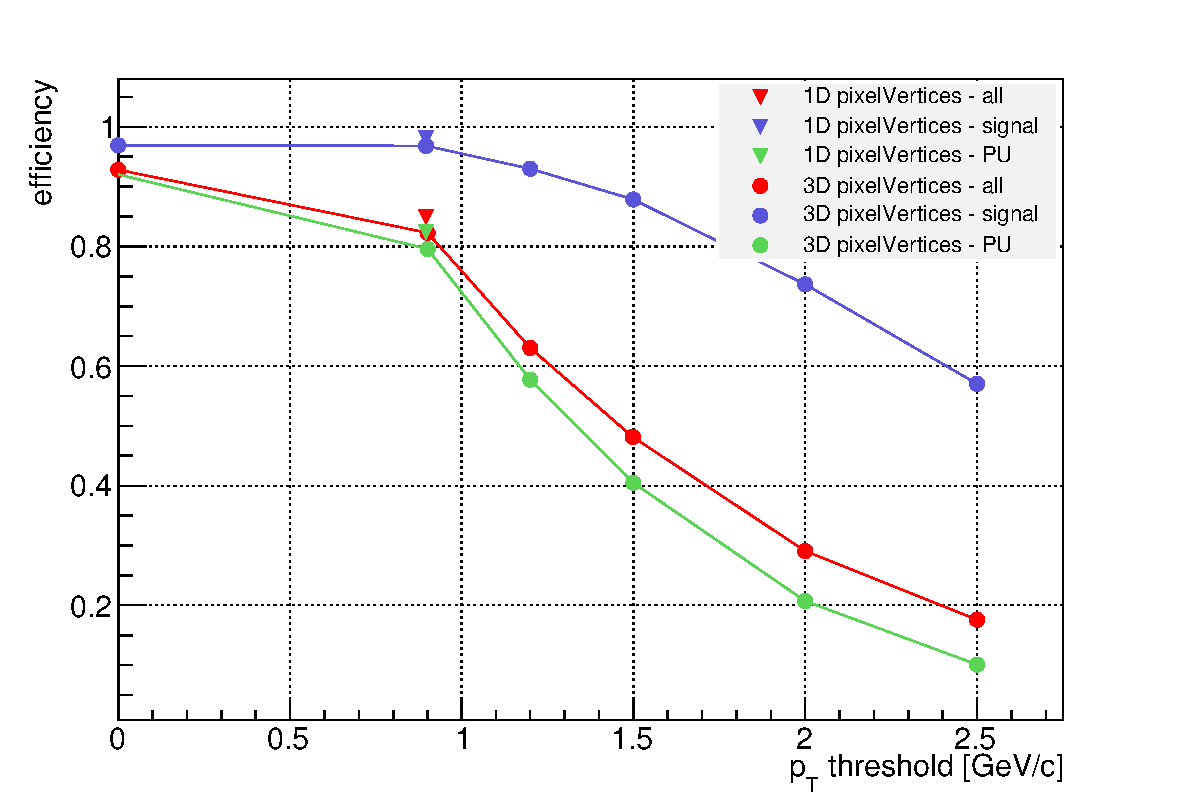
\includegraphics[height=4.7cm]{figures/3DPVeff.pdf}}
   \hspace{0.1cm}
   %%----start of second subfigure----
   \subfloat[]{
     \label{faker}           %% label for second subfigure
        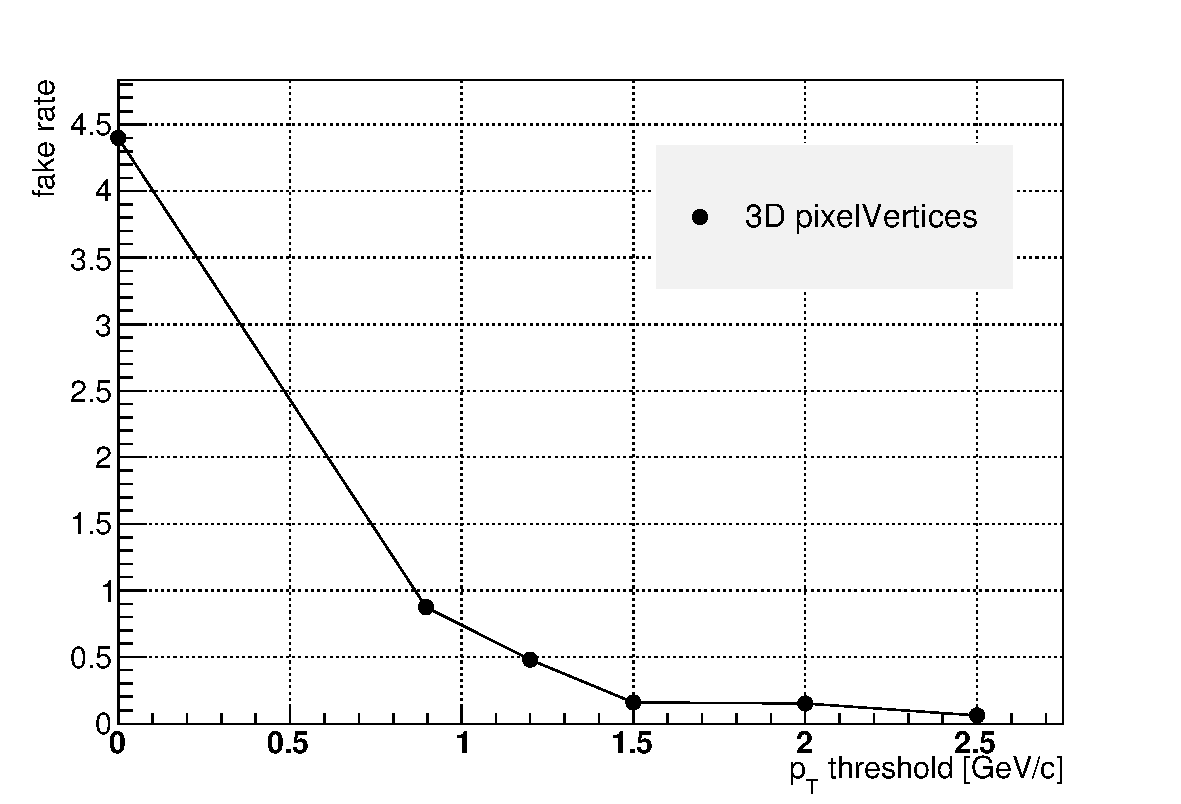
\includegraphics[height=4.7cm]{figures/3DPVfake.pdf}}
   \caption{\small{(a) primary vertex finding efficiency provided by the 3D reconstruction, for all vertices in the event, and separately for signal and pile up vertices, as a function of the $p_{T}$ threshold applied in the pixel track selection. The result for the 1D pixel vertex reconstruction is also shown for a comparison. (b) rate of fake vertices in the event, as a function of the $p_{T}$ threshold. The corresponding fake rate for the 1D reconstruction is 12.5\% for a $p_{T}$ cut of 0.9 GeV$/c$.}}
   \label{efffake}                  %% label for entire figure
\end{figure}
%_________________________________________________________________________________
\begin{figure}
   \centering
   %%----start of first subfigure----
   \subfloat[]{
        \label{resT}           %% label for first subfigure
        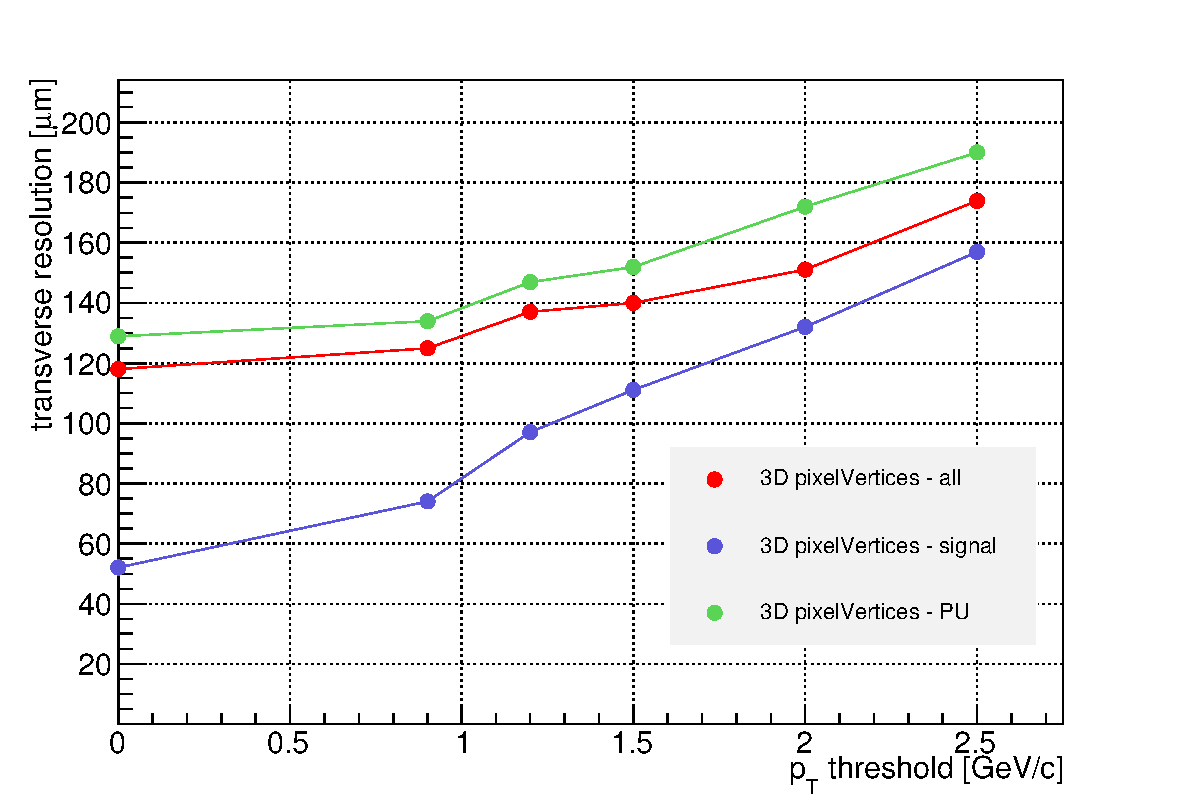
\includegraphics[height=4.7cm]{figures/3DPVresX.pdf}}
   \hspace{0.1cm}
   %%----start of second subfigure----
   \subfloat[]{
     \label{resL}           %% label for second subfigure
        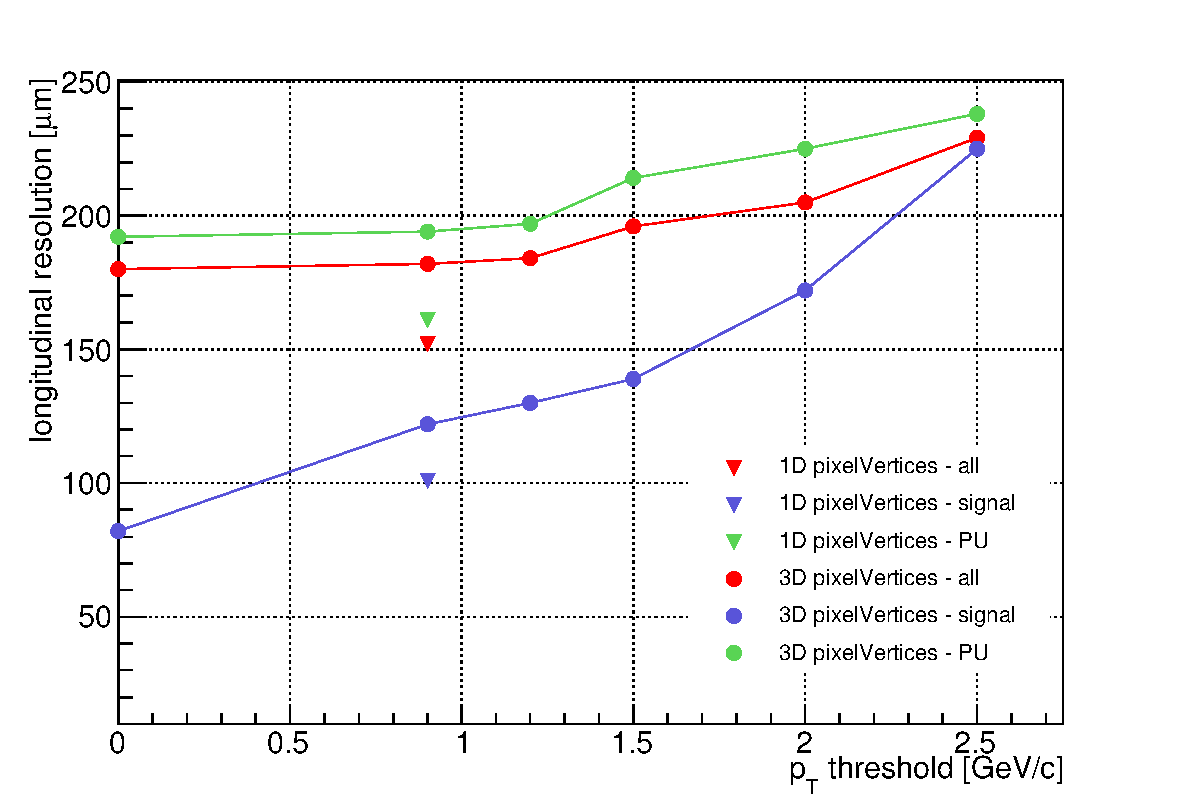
\includegraphics[height=4.7cm]{figures/3DPVresL.pdf}}
   \caption{\small{(a) transverse and (b) longitudinal 3D primary vertex position resolution as a function of the $p_{T}$ threshold applied in the pixel track selection. In (b) the result for the 1D reconstruction is also shown for comparison.}}
   \label{res}                  %% label for entire figure
\end{figure}
From Fig.\ref{eff} it is evident that a working point for this algorithm should be chosen in the region up to about 1.2 GeV$/c$, where the signal vertex efficiency is higher than 90\%, and competitive with the 1D reconstruction. The fake rate in this range is between 4.5\% and 0.5\%, to be compared to 12.5\% that we obtain for the 1D reconstruction. For the signal vertex, the longitudinal position resolution ranges between 80 and 120 $\mu$m. The transverse resolution is between two and four times worse than the beamspot width (about 25 $\mu$m), which is the limitation of the 1D algorithm. This should still assure sufficiently good b-tagging performance for the purpose of the online event selection. \\
A summary of the 3D vertex reconstruction performance is given in Table \ref{summary}, together with an estimation of the running time (CPU) of the module. 
\begin{table}[htbp]
\begin{center}
\begin{tabular}{|c|c|}
\hline
$p_{T}$ threshold (GeV$/c$) & running time (ms) \\
\hline
no threshold & 32.6 \\
0.9 & 15.5 \\
1.2 & 10.0 \\
1.5 & 7.1 \\
2.0 & 4.8 \\
2.5 & 3.9 \\
\hline
\end{tabular}
\end{center}
\caption{Running time (CPU) of the 3D primary vertex producer module as a function of the $p_{T}$ threshold applied in the pixel track selection.} 
\label{summary}
\end{table}

\clearpage
\section{Data and Monte Carlo samples, reconstruction and selection \label{sec:samples}}
Monte Carlo Samples have been generated with PYTHIA6, tune Z2, in several bins of $\hat{p}_T$. Table \ref{tab:MCsamples} shows the names of the MC samples, and the number of processed events. The pileup conditions in data change rapidly so the Monte Carlo cannot be expected to match the data exactly. The Monte Carlo samples have therefore been gererated with a flat pileup distribution including a poissonian tail. This scenario covers roughtly the conditions of the 2011 run. The residual differences in pileup conditions are taken into account with a reweighting procedure as explained later in this section. The samples in Table \ref{tab:MCsamples} have been used for the main commissioning and validation studies in Sections \ref{sec:impactparameter} to \ref{sec:discriminators}. Another set of samples requiring the presence of a muon at generator level has been produced for the studies of muon jets  in Section~\ref{sec:muonjets}. The details of the muon enriched samples are given in Table~\ref{tab:MCsampleMuEnriched}.

\begin{table}[h!]
\caption{QCD Monte Carlo samples. All sample names have to be extended with the suffix /Spring11-PU\_S1\_START311\_V1G1-v1/AODSIM.}
\centering
\begin{tabular}{| l | l |}
\hline
sample &  \# events \\
\verb|/QCD_Pt_5to15_TuneZ2_7TeV_pythia6|     & 3296192 \\
\verb|/QCD_Pt_15to30_TuneZ2_7TeV_pythia6|    & 8213600 \\
\verb|/QCD_Pt_30to50_TuneZ2_7TeV_pythia6|    & 6529320 \\
\verb|/QCD_Pt_50to80_TuneZ2_7TeV_pythia6|    & 4301392 \\
\verb|/QCD_Pt_80to120_TuneZ2_7TeV_pythia6|   & 6407732 \\
\verb|/QCD_Pt_120to170_TuneZ2_7TeV_pythia6|  & 6090400 \\
\verb|/QCD_Pt_170to300_TuneZ2_7TeV_pythia6|  & 5684160 \\
\verb|/QCD_Pt_300to470_TuneZ2_7TeV_pythia6|  & 6336960 \\
\hline
\end{tabular}
\label{tab:MCsamples}
\end{table}

\begin{table}[h!]
\caption{Muon Enriched Monte Carlo samples. All sample names have the suffix /Spring11-PU\_S1\_START311\_V1G1-v1/AODSIM.}
\centering
\begin{tabular}{| l | l |}
\hline
sample &  \# events \\
\verb|/QCD_Pt-15to20_MuPt5Enriched_TuneZ2_7TeV-pythia6|   & 2884915  \\
\verb|/QCD_Pt-20to30_MuPt5Enriched_TuneZ2_7TeV-pythia6|   & 11352301 \\
\verb|/QCD_Pt-30to50_MuPt5Enriched_TuneZ2_7TeV-pythia6|   & 10909951 \\
\verb|/QCD_Pt-50to80_MuPt5Enriched_TuneZ2_7TeV-pythia6|   & 10686315 \\
\verb|/QCD_Pt-80to120_MuPt5Enriched_TuneZ2_7TeV-pythia6|  & 3183540  \\
\verb|/QCD_Pt-120to150_MuPt5Enriched_TuneZ2_7TeV-pythia6| & 991024   \\
\verb|/QCD_Pt-150_MuPt5Enriched_TuneZ2_7TeV-pythia6|      & 1015900  \\
\hline
\end{tabular}
\label{tab:MCsampleMuEnriched}
\end{table}




We use "Particle Flow Jets" (PFjets) \cite{bib:particleFlow} using the anti-$k_T$ jet clustering method \cite{AntiKT} with cone radius parameter $\Delta R = \sqrt{\Delta \eta^2 + \Delta \phi^2} = 0.5$. In addition, ``L2L3'' Jet energy corrections and the following   jet ID cuts are applied:
\begin{verbatim}
pt > 10.0 && abs(eta) < 2.5 && neutralHadronEnergyFraction < 1.0 && 
neutralEmEnergyFraction < 1.0  && nConstituents > 1 && 
chargedHadronEnergyFraction > 0.0 && chargedMultiplicity > 0.0 && 
chargedEmEnergyFraction < 1.0
\end{verbatim}
The jet ID cuts are introduced after the L2L3 energy corrections.


Tracks are reconstructed using the standard CMS iterative tracking procedure. The Combinatorial
Kalman Filter algorithm \cite{CMS_PTDR_1, CMSTRK10001, CMS_PAS_TRK-10-005}  is applied in an iterative way with increasingly relaxed impact parameter constraint and different seeding layers. 

The primary vertex (PV) is reconstructed from all  tracks in the event which are compatible with the beam spot. The new ``Deterministic Annealing Filter'' (DA) algorithm is used for PV reconstruction ({\bf FIXME: reference plus more details})

The CMSSW software version 4.1.6 is used to analyze the Monte Carlo samples. This version has been patched with a backport of the DA primary vertex reconstructor and a fixed version of the secondary vertex producer. Data samples are analyzed with CMSSW 4.2.3 without any additional patches.

The commissioning studies in Sections \ref{sec:impactparameter} to \ref{sec:discriminators} are using a single jet trigger \verb|HLT_Jet60| for data, while the trigger \verb|HLTJet30U| is applied in Monte Carlo samples.  A jet $p_t$ threshold of 60~GeV is applied both in data and Monte Carlo. It has been verified that the resulting jet $p_t$ spectra are in reasonable agreement between data and Monte Carlo.

The studies requiring muons in jets have been made applying the jet+muon di-jet trigger \verb|HLT_BTagMu_DiJet40_Mu5| in data. Both in data and Monte Carlo, the requirement of two jets with $p_t > 60$ and one jet with $p_t > 65$ GeV is applied. Muons are required to have transverse momentum $p_t >$ 7 GeV.

In addition, another set of validation plots are produced with lower trigger threshold (\verb|HLT_Jet30| in data and \verb|HLTJet15U| in Monte Carlo)  and lower jet momentum cut of $p_t >$ 30 GeV in case of the single jet triggers. For the b-jet triggers another set of plots has been produced with \verb|HLT_BTagMu_DiJet20_Mu5|, requiring two jets with $p_t >$ 40 GeV, one of them with $p_t >$ 45 GeV. Details are given in Appendix \ref{sec:AppendixA}.

An overview of the used data samples, triggers and effective integrated luminosity (including trigger prescales) is given in Table \ref{tab:dataSamples}.

\begin{tabular}{| l | l | l |}
\hline
sample &  trigger & effective lumi \\
\verb|/Jet/Run2011A-PromptReco-v1(v2)|      & \verb|HLT_Jet30|              & $3.06 \cdot 10^{-3}$ pb$^{-1}$ \\
\verb|/Jet/Run2011A-PromptReco-v1(v2)|      & \verb|HLT_Jet60|              & 0.056 pb$^{-1}$ \\
\verb|/METBTag/Run2011A-PromptReco-v1(v2)|  & \verb|HLT_BTagMu_DiJet20_Mu5| & 1.62 pb$^{-1}$ \\
\verb|/METBTag/Run2011A-PromptReco-v1(v2)|  & \verb|HLT_BTagMu_DiJet40_Mu5| & 3.12 pb$^{-1}$ \\
\hline
\end{tabular}
\label{tab:dataSamples}
\end{table}

The number of reconstructed primary vertices is shown in Section \ref{sec:pileup}. It is visible that Monte Carlo does not describe the pileup multiplicity correctly. We therefore apply a vertex reweighting procedure in which all distributions obtained from Monte Carlo are reweighted so that the vertex multiplicity agrees between data and Monte Carlo. This reweighting procedure has been applied for all distributions in Sections \ref{sec:impactparameter} to \ref{sec:muonjets}.



\section{Track selection \label{sec:trackselection}}
Tracks are associated to jets using a cone in $\eta - \phi$ space defined as $\Delta R = \sqrt{\Delta \eta^2 + \Delta \phi^2} < 0.5$. A new development which introduces a variable cone size is discussed in Section~\ref{sec:dvelopments}. 

Furhter selection criteria for tracks are listed in the following. The corresponding distributions for all tracks within a distance $\Delta R < 0.5$ to the jet axis are displayed in Figures~\ref{fig:inputVars1} to \ref{fig:inputVars3}.
\begin{itemize}
\item number of pixel hits $>= 2$  (Figure \ref{fig:inputVars1})
\item number of tracker hits (including pixel) $>= 8$ (Figure \ref{fig:inputVars1})
\item transverse impact parameter $|IP_{2D}| < 0.2$~cm (Figure \ref{fig:inputVars1})
\item transverse momentum $p_t > 1$~GeV/$c$ (Figure \ref{fig:inputVars2})
\item normalized $\chi^2 < 5$ (Figure \ref{fig:inputVars2})
\item longitudinal impact parameter $|IP_{z}|< 17$~cm (Figure \ref{fig:inputVars2})
\item distance to jet axis $ < 0.07$~cm (Figure \ref{fig:inputVars3})
\item decay length $< 5$ (Figure \ref{fig:inputVars3})
\end{itemize}
Figures~\ref{fig:inputVars1} to \ref{fig:inputVars3} show the track selection variables without any cuts, while Figures~\ref{fig:inputVars1N} to \ref{fig:inputVars3N} show the same variables but with all cuts, except for the cut on the variable displayed ($n$-1 cuts).
\begin{figure}[h!]
\centering
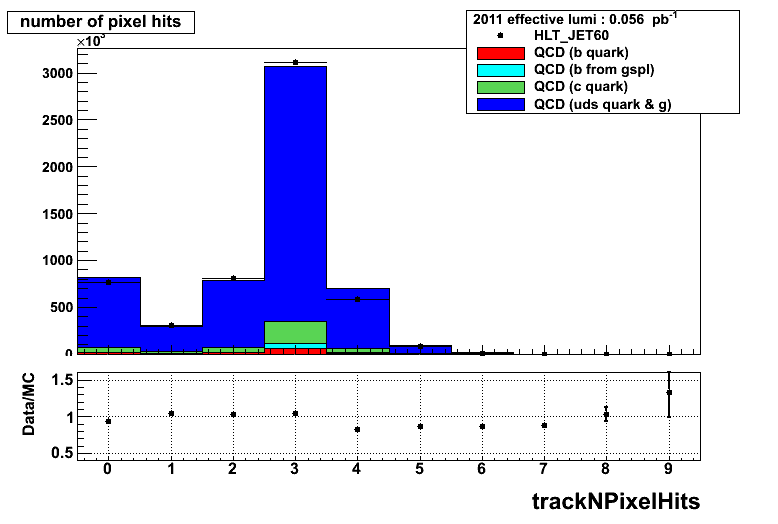
\includegraphics[width=0.32\textwidth]{figures/trackNPixelHits_Linear.png}
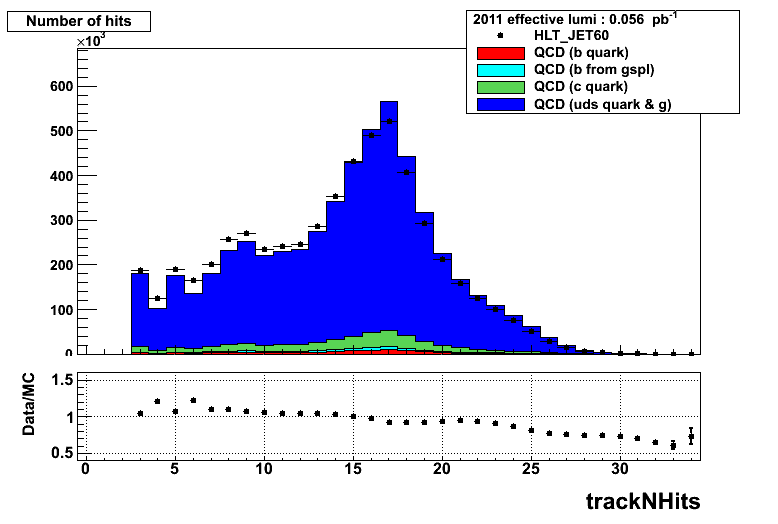
\includegraphics[width=0.32\textwidth]{figures/trackNHits_Linear.png}
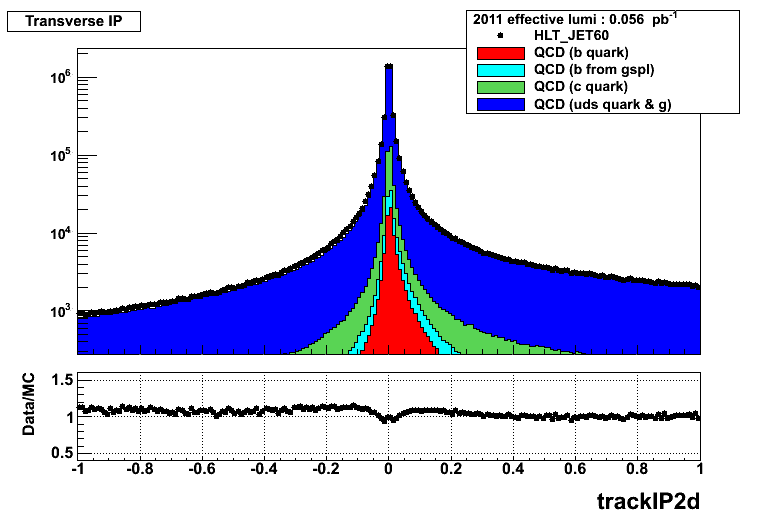
\includegraphics[width=0.32\textwidth]{figures/trackIP2d_Log.png}
\caption{Left: number of hits in the pixel detector, middle: total number of hits in the tracker, right: transverse track impact parameter. No cuts on  track variables were applied.}
\label{fig:inputVars1}
\end{figure}

\begin{figure}[h!]
\centering
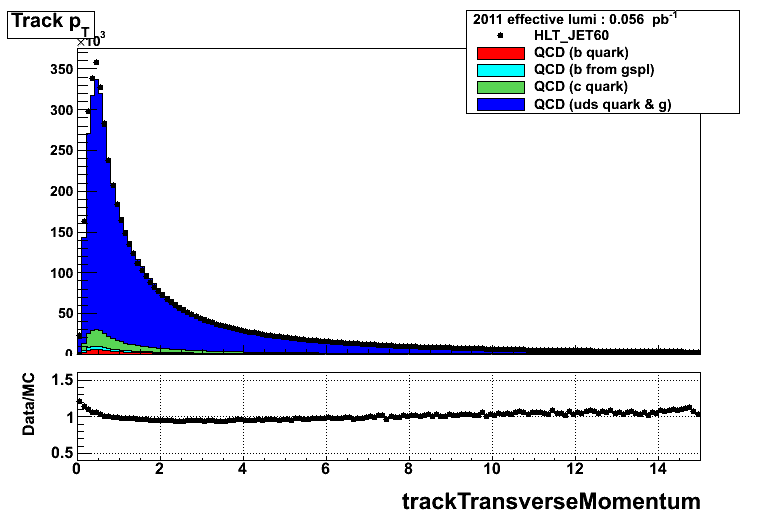
\includegraphics[width=0.32\textwidth]{figures/trackTransverseMomentum_Linear.png}
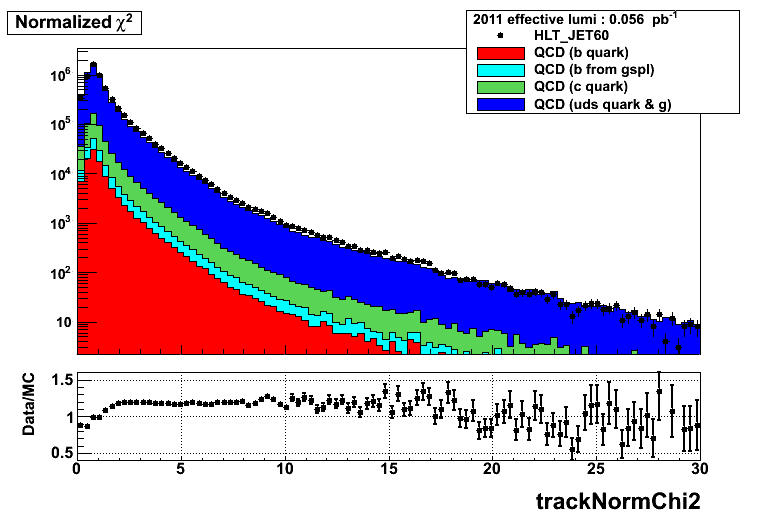
\includegraphics[width=0.32\textwidth]{figures/trackNormChi2_Log.png}
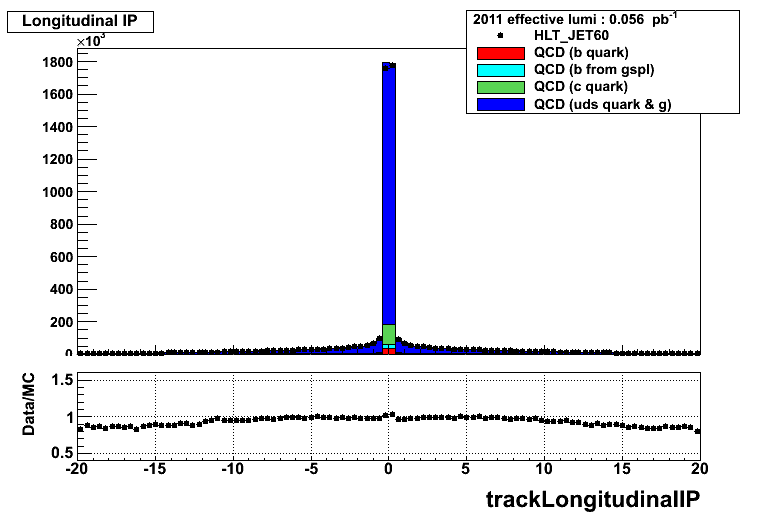
\includegraphics[width=0.32\textwidth]{figures/trackLongitudinalIP_Linear.png}
\caption{Left: transverse track momentum, middle: normalized track $\chi^2$, right: longitudinal impact parameter.  No cuts on track variables were applied.}
\label{fig:inputVars2}
\end{figure}

\begin{figure}[h!]
\centering
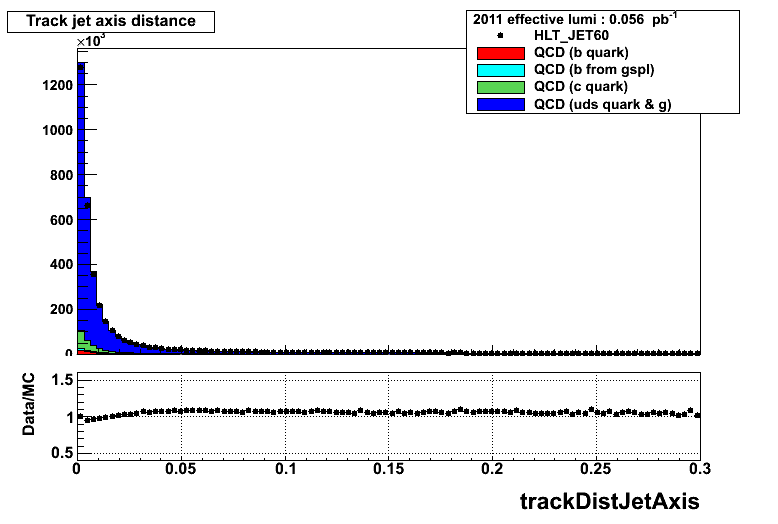
\includegraphics[width=0.42\textwidth]{figures/trackDistJetAxis_Linear.png}
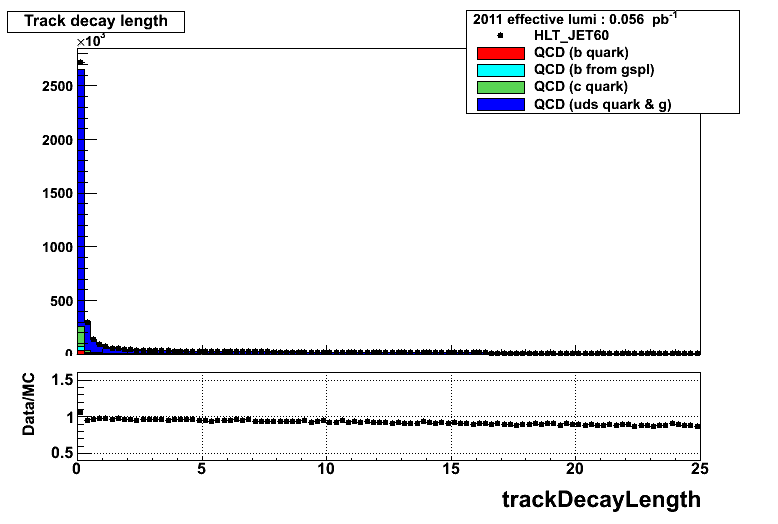
\includegraphics[width=0.42\textwidth]{figures/trackDecayLength_Linear.png}
\caption{Left: distance to jet axis, right: track decay length.  No cuts on track variables were applied. }
\label{fig:inputVars3}
\end{figure}

\begin{figure}[h!]
\centering
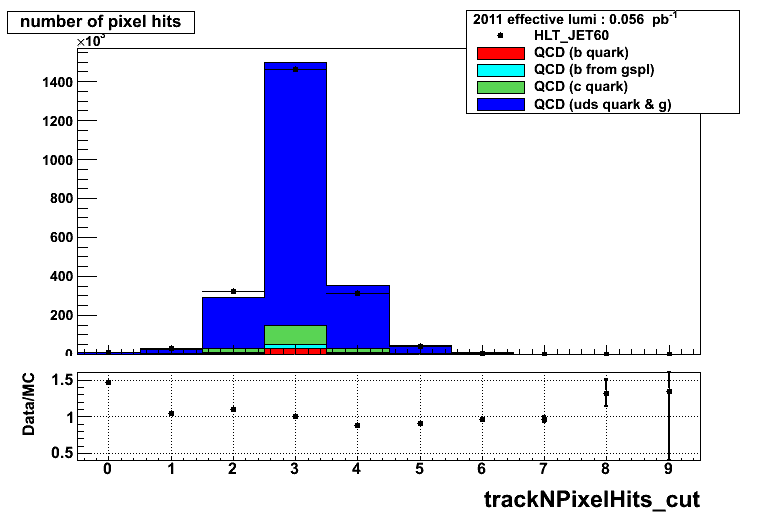
\includegraphics[width=0.32\textwidth]{figures/trackNPixelHits_cut_Linear.png}
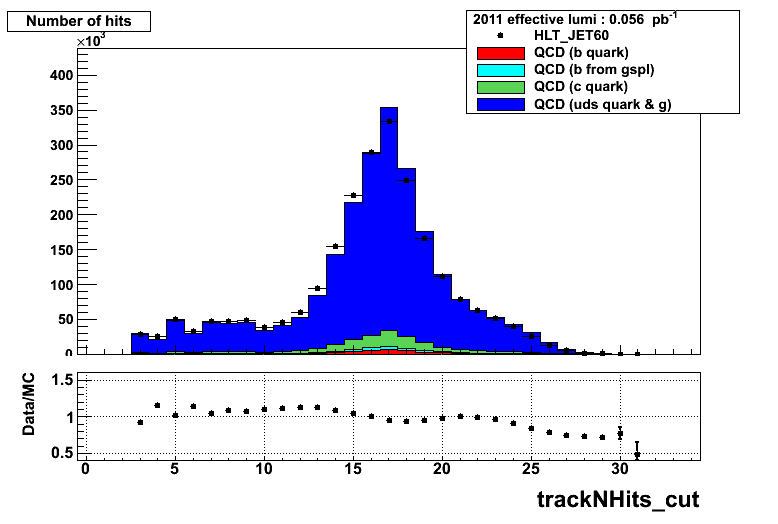
\includegraphics[width=0.32\textwidth]{figures/trackNHits_cut_Linear.png}
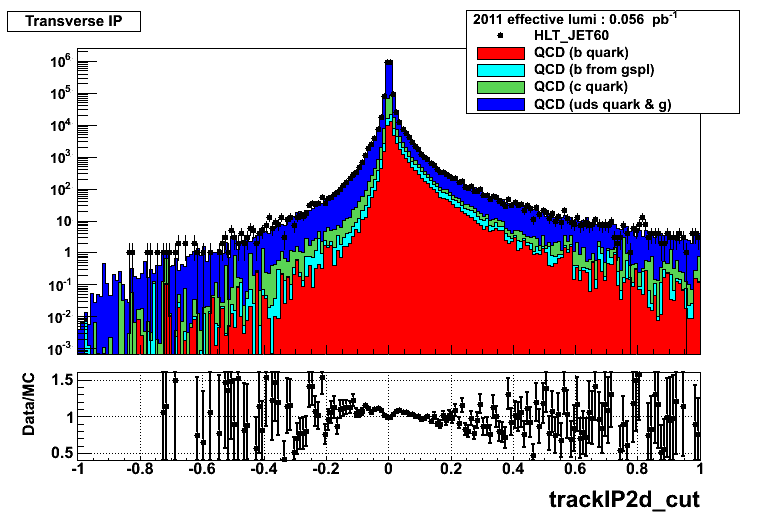
\includegraphics[width=0.32\textwidth]{figures/trackIP2d_cut_Log.png}
\caption{Left: number of hits in the pixel detector, middle: total number of hits in the tracker, right: transverse track impact parameter.  All cuts on track selection variables were applied, except for the cut on the displayed quantity.}
\label{fig:inputVars1N}
\end{figure}

\begin{figure}[h!]
\centering
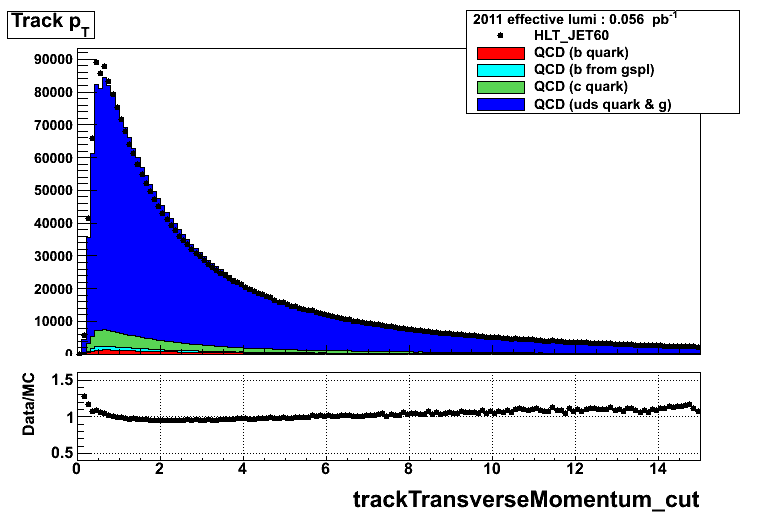
\includegraphics[width=0.32\textwidth]{figures/trackTransverseMomentum_cut_Linear.png}
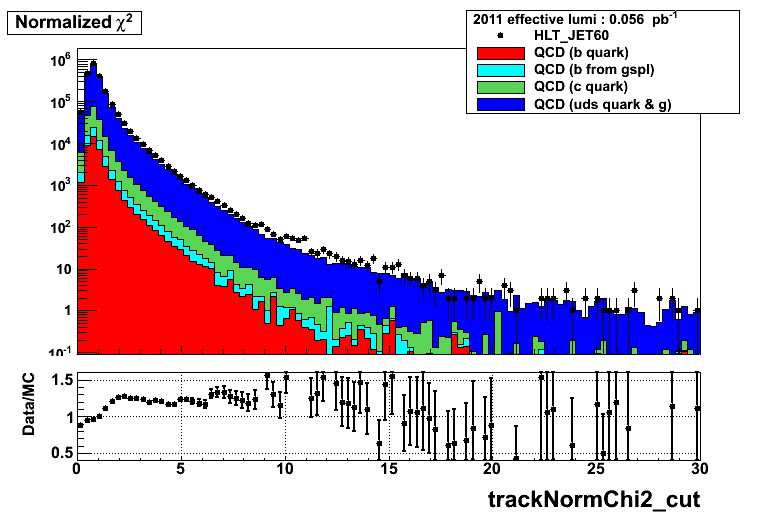
\includegraphics[width=0.32\textwidth]{figures/trackNormChi2_cut_Log.png}
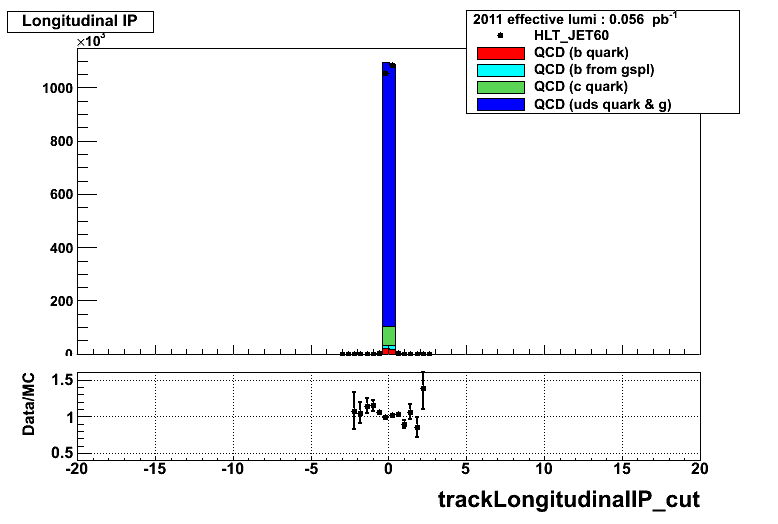
\includegraphics[width=0.32\textwidth]{figures/trackLongitudinalIP_cut_Linear.png}
\caption{Left: transverse track momentum, middle: normalized track $\chi^2$, right: longitudinal impact parameter.   All cuts on track selection variables were applied, except for the cut on the displayed quantity.}
\label{fig:inputVars2N}
\end{figure}

\begin{figure}[h!]
\centering
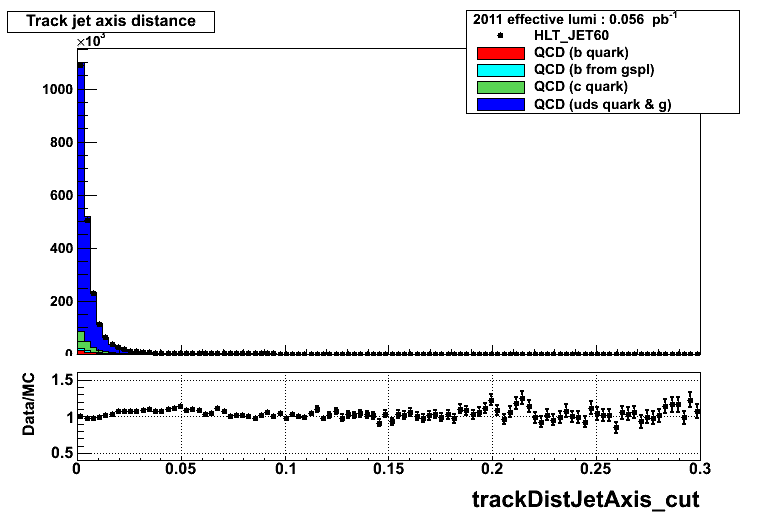
\includegraphics[width=0.42\textwidth]{figures/trackDistJetAxis_cut_Linear.png}
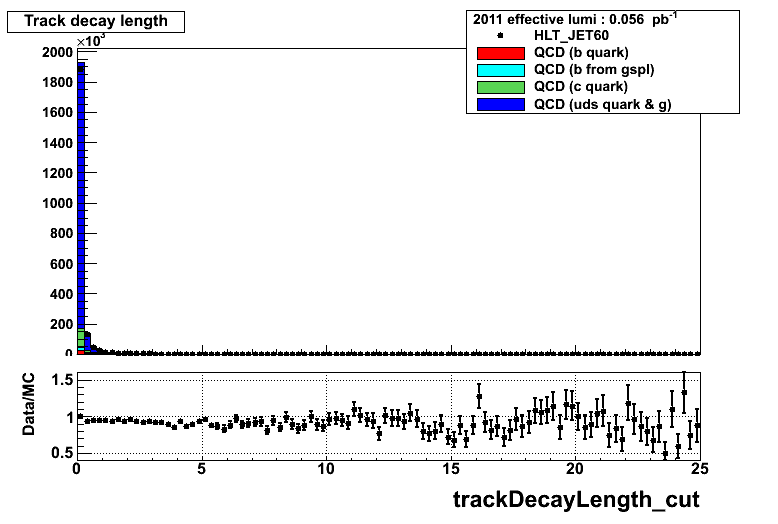
\includegraphics[width=0.42\textwidth]{figures/trackDecayLength_cut_Linear.png}
\caption{Left: distance to jet axis, right: track decay length.  All cuts on track selection variables were applied, except for the cut on the displayed quantity. }
\label{fig:inputVars3N}
\end{figure}



This track selection is used for all impact parameter based algorithms, i.e. the track counting and track probability algorithms. The secondary vertex based algorithms apply slightly different selection criteria (only those which are different are listed in the following):
\begin{itemize}
\item jet-track association cone $\Delta R < 0.3$
\item distance to jet axis $ < 0.2$~cm
\item no cut on decay length
\item track quality class = "high purity" 
\end{itemize}

The average number of tracks per jet is displayed in Figure~\ref{fig:trackMult} 
for the case with and without track selection cuts.  The average number of tracks also depends on the jet energy which is shown in Figure~\ref{fig:trackMultVsPt}. The discrepancy between data and simulation is attributed to the Monte Carlo event generator which is not reproducing the charged particle kinematics perfectly.


\begin{figure}[h!]
\centering
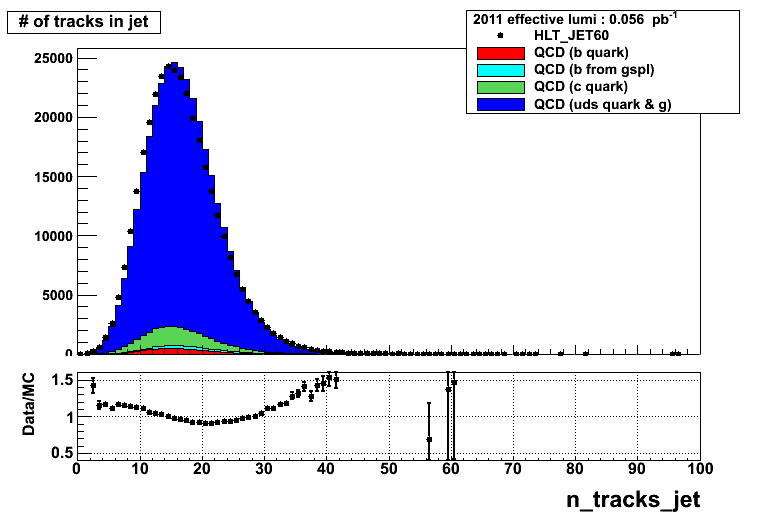
\includegraphics[width=0.42\textwidth]{figures/n_tracks_jet_Linear.png}
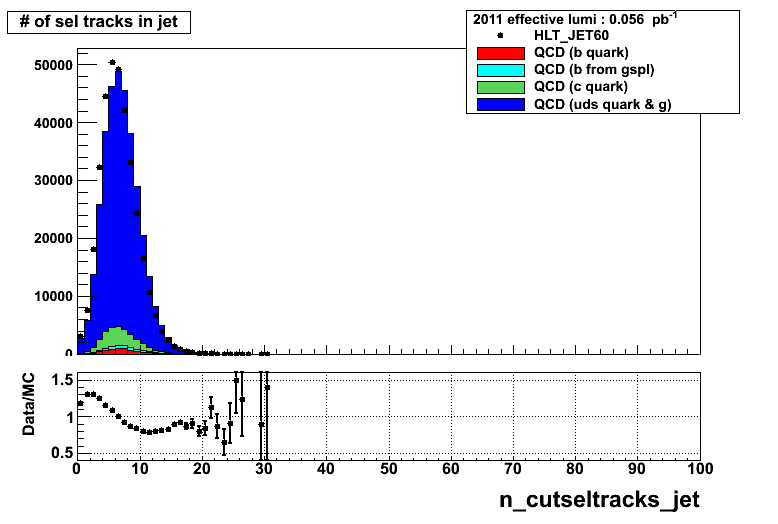
\includegraphics[width=0.42\textwidth]{figures/n_cutseltracks_jet_Linear.png}
\caption{Left: number of tracks within $\Delta R < 0.5$ of the jet axis. Right: the same for tracks passing the selection criteria of the IP based algorithms as explained in the text.}
\label{fig:trackMult}
\end{figure}

\begin{figure}[h!]
\centering
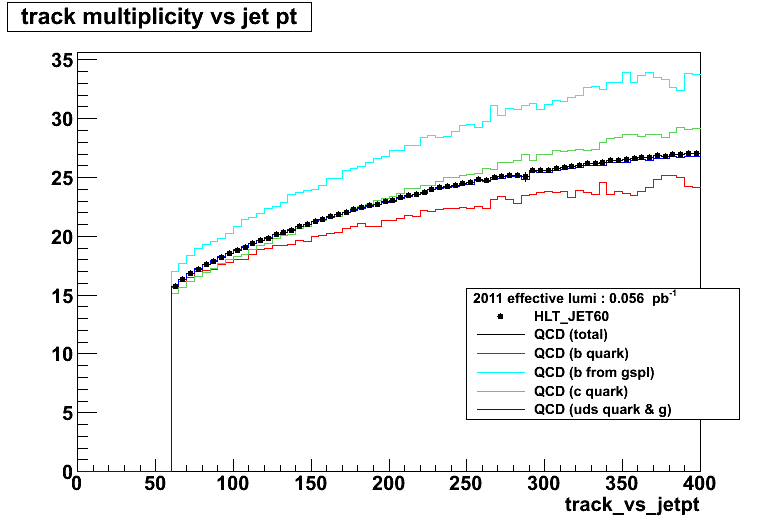
\includegraphics[width=0.42\textwidth]{figures/track_vs_jetpt_Linear.png}
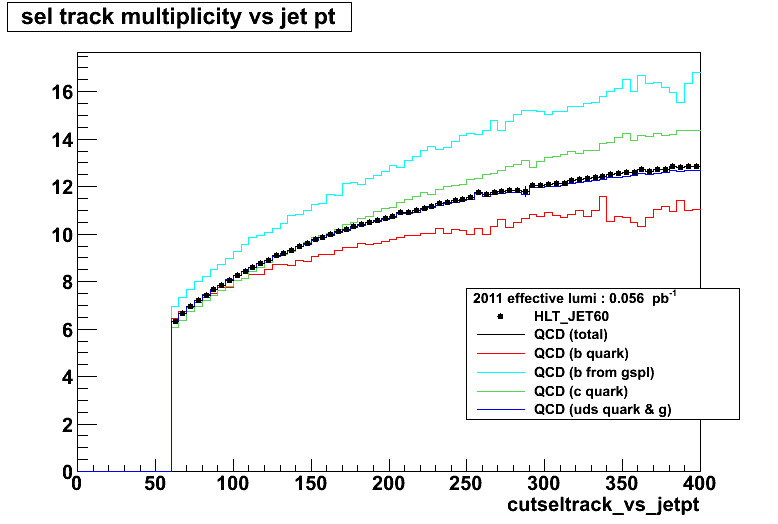
\includegraphics[width=0.42\textwidth]{figures/cutseltrack_vs_jetpt_Linear.png}
\caption{Left: average number of tracks associated to a jet depending on transverse jet momentum $p_t$. Right:  average number of selected tracks associated to a jet depending on transverse jet momentum $p_t$.}
\label{fig:trackMultVsPt}
\end{figure}

\clearpage
\section{Impact parameter \label{sec:impactparameter}}
The impact parameter (IP) is defined as the minimum distance between
the primary vertex and the trajectory of the track. Tracks produced by
long lived particles such as B mesons are expected to have a sizable
IP.  In the ultra-relativistic limit the IP is Lorentz-invariant to a
good approximation due to the cancellation of boost effects and the
angle of the decay products with respect to the flight path. The
precision of the IP measurement can be different from track to track
and is between 30~$\mu$m and several hundreds $\mu$m. Given that the
uncertainty can be of the same order as the IP value, the IP
significance $S= IP/\sigma_{IP}$ is used for tagging b-jets. 

The IP is ``lifetime signed'': tracks originating from the decay of
particles traveling in the same direction of the jet are signed as
positive, while those in opposite direction are tagged as
negative. This is obtained by using the sign of the scalar product of
the IP segment with the jet direction. It should be noted that a ``sign
flip'' can happen to track produced in the region between the jet
direction and the actual B-hadron flight direction. 


The IP can be measured either in the transverse plane only or in three
dimensions. The high resolution of the pixel detector also along the z
coordinate allows the use of the 3D IP: despite the precision in z being slightly inferior with respect to the one in the
transverse plane, by using the 3D significance the precision is not 
spoiled as the measurement errors are correctly taken into account.   
 

3D Impact Parameter value, error and significance for first, second and
third track in the jet (ordered by IP significance) are displayed in
Figures~\ref{fig:IPfirstTrack} to \ref{fig:IPThirdTrack}. Figure
\ref{fig:IPAllTrack} shows the same for all selected tracks in a jet
(i.e. not ordered by IP significance).

\begin{figure}[h!]
\centering
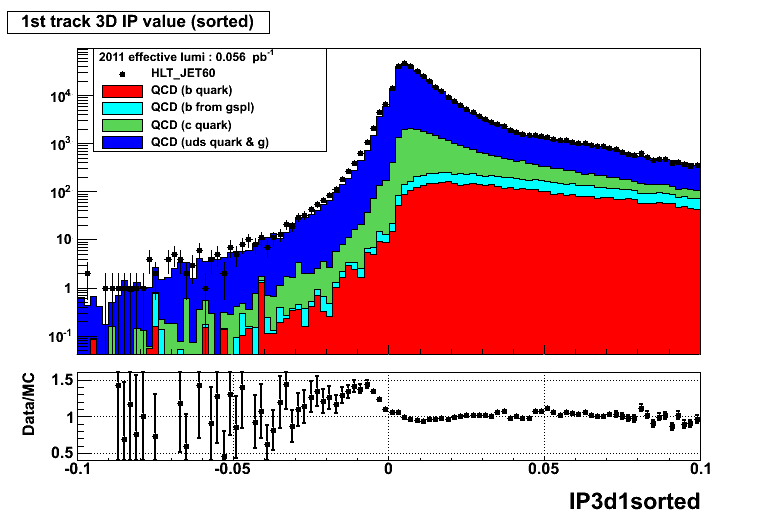
\includegraphics[width=0.32\textwidth]{figures/IP3d1sorted_Log.png}
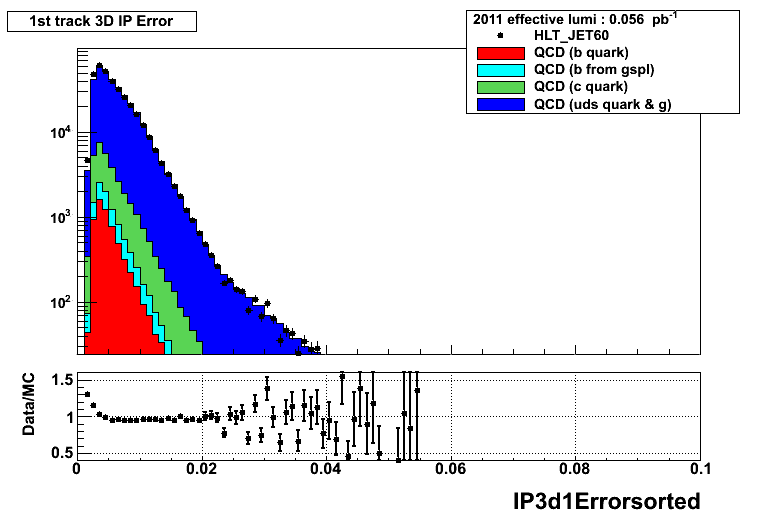
\includegraphics[width=0.32\textwidth]{figures/IP3d1Errorsorted_Log.png}
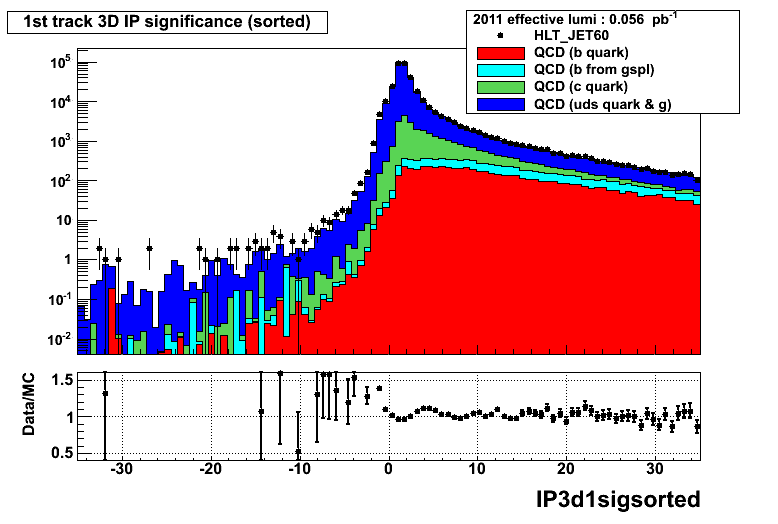
\includegraphics[width=0.32\textwidth]{figures/IP3d1sigsorted_Log.png}
\caption{Left: IP value, middle: IP error, right: IP significance for the first track in the jet, ordered by IP significance.  }
\label{fig:IPfirstTrack}
\end{figure}

\begin{figure}[h!]
\centering
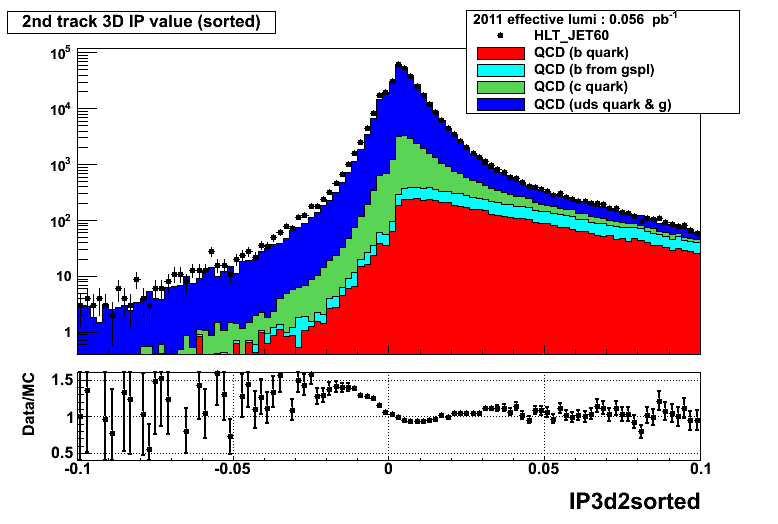
\includegraphics[width=0.32\textwidth]{figures/IP3d2sorted_Log.png}
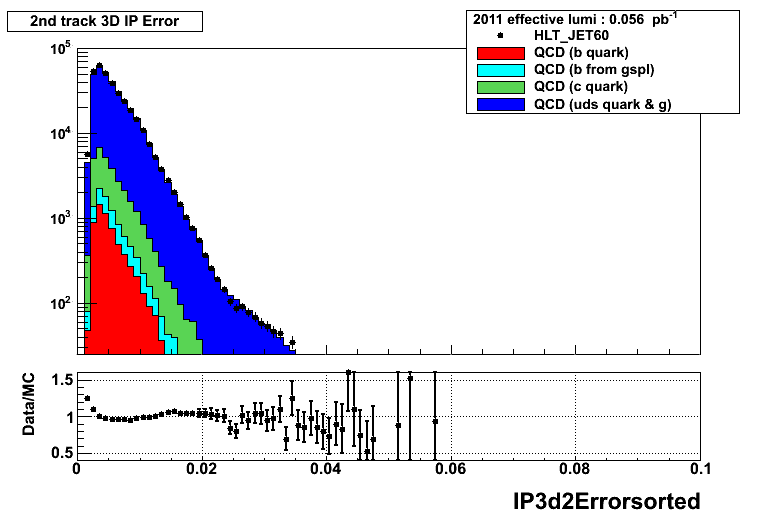
\includegraphics[width=0.32\textwidth]{figures/IP3d2Errorsorted_Log.png}
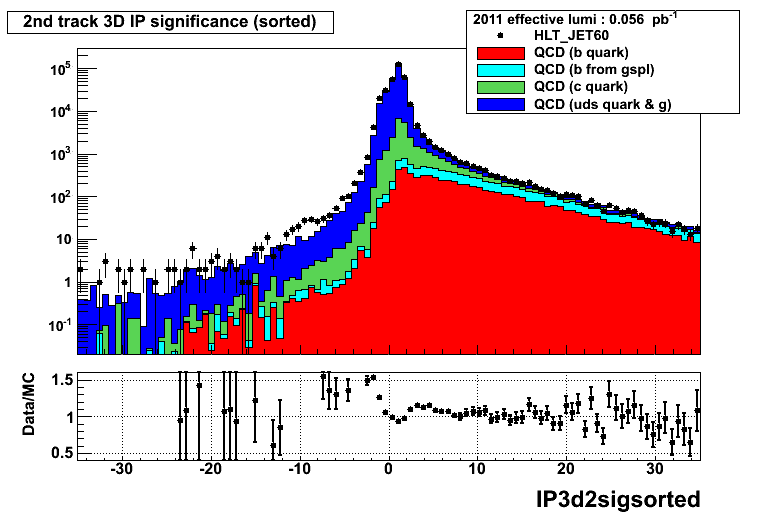
\includegraphics[width=0.32\textwidth]{figures/IP3d2sigsorted_Log.png}
\caption{Left: IP value, middle: IP error, right: IP significance for the second track in the jet, ordered by IP significance.  }
\label{fig:IPsecondTrack}
\end{figure}

\begin{figure}[h!]
\centering
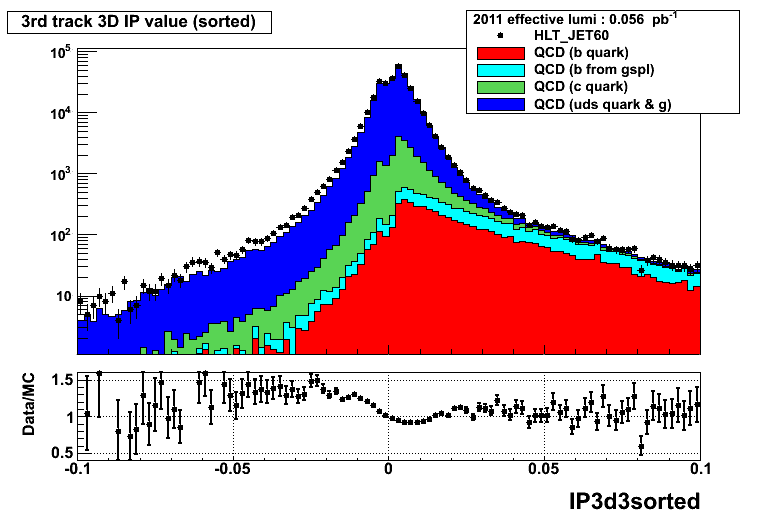
\includegraphics[width=0.32\textwidth]{figures/IP3d3sorted_Log.png}
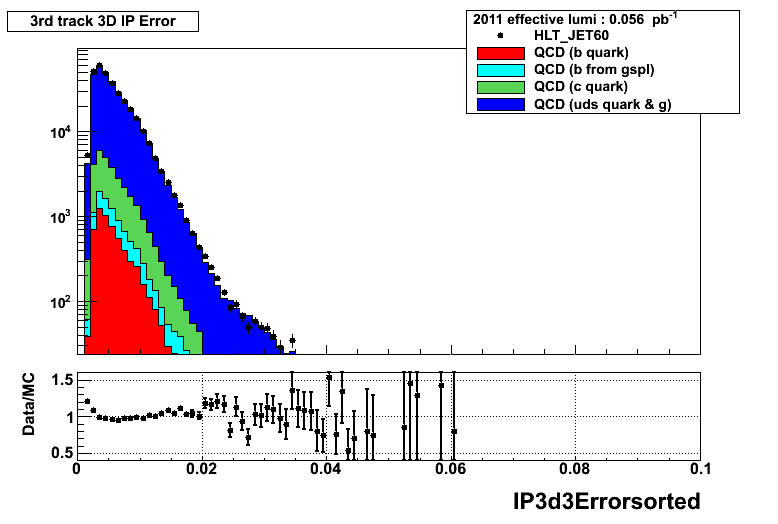
\includegraphics[width=0.32\textwidth]{figures/IP3d3Errorsorted_Log.png}
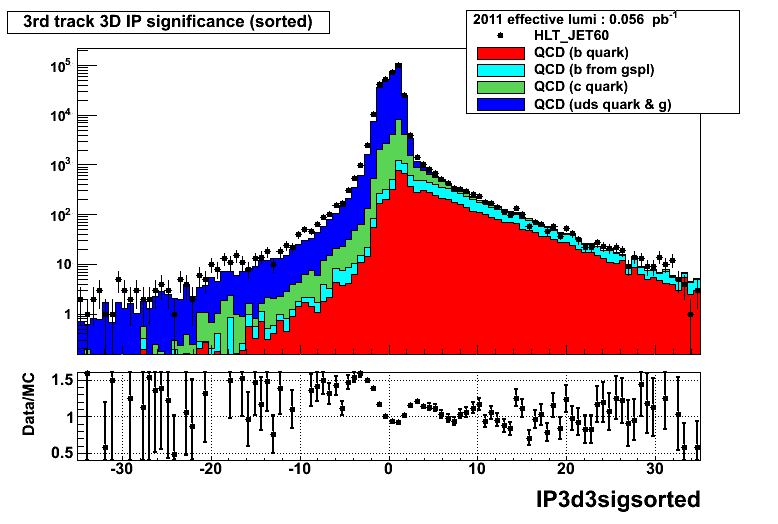
\includegraphics[width=0.32\textwidth]{figures/IP3d3sigsorted_Log.png}
\caption{Left: IP value, middle: IP error, right: IP significance for the third track in the jet, ordered by IP significance.  }
\label{fig:IPThirdTrack}
\end{figure}

\begin{figure}[h!]
\centering
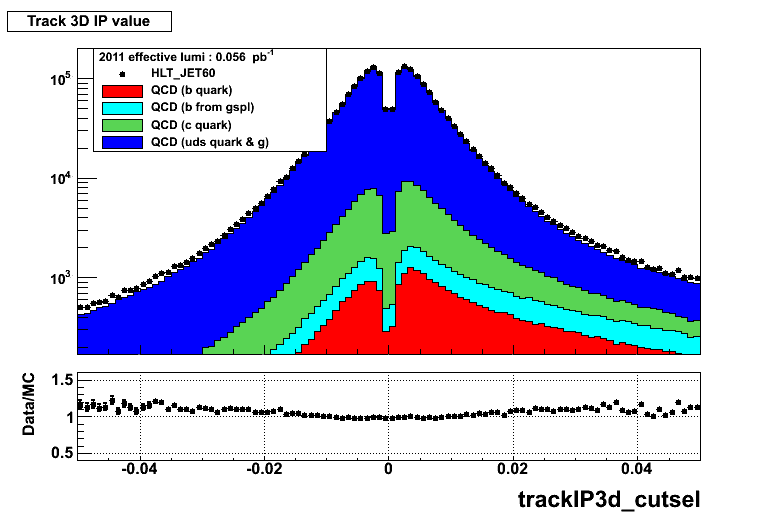
\includegraphics[width=0.32\textwidth]{figures/trackIP3d_cutsel_Log.png}
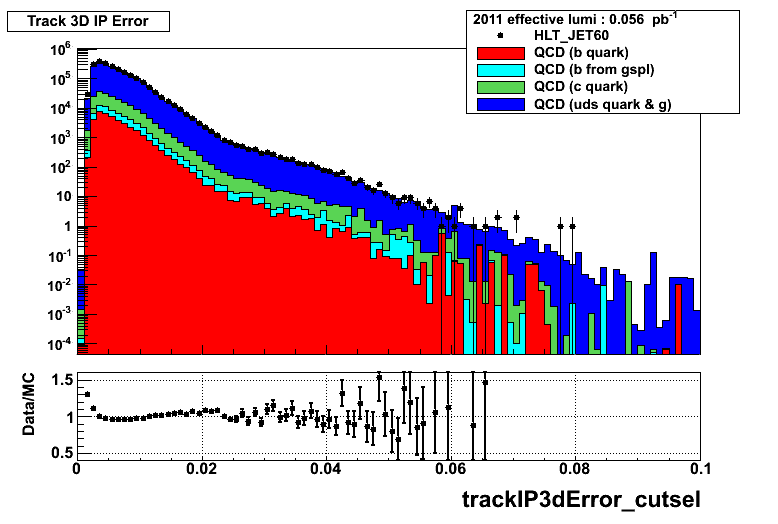
\includegraphics[width=0.32\textwidth]{figures/trackIP3dError_cutsel_Log.png}
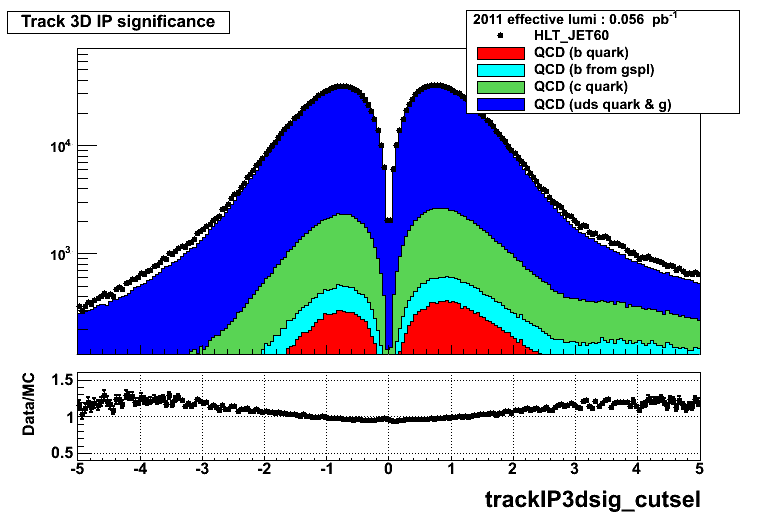
\includegraphics[width=0.32\textwidth]{figures/trackIP3dsig_cutsel_Log.png}
\caption{Left: IP value, middle: IP error, right: IP significance for all selected tracks in the jet. The track selection as defined in Section~\ref{sec:trackselection} has been applied.}
\label{fig:IPAllTrack}
\end{figure}



The impact parameter has slightly different behaviour depending on the track momentum. This is shown in Figure~\ref{fig:IPbinnedTrackpt} which displays the track IP values for six different track $p_t$ bins.  

% A major source of discrepancies is the number of tracks associated to the jets. This is visible in Figure~\ref{fig:IPBinnedInNtracks} which shows the first track $p_t$ bin split into nince bins of number of tracks per jet.



\begin{figure}[h!]
\centering
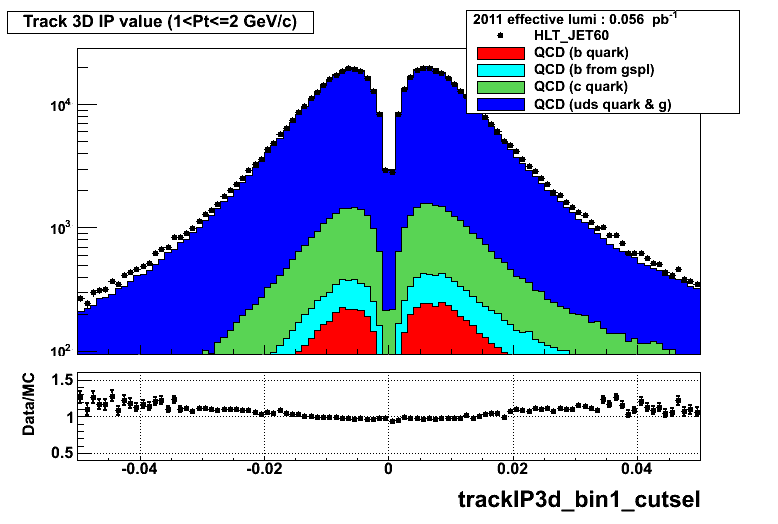
\includegraphics[width=0.32\textwidth]{figures/trackIP3d_bin1_cutsel_Log.png}
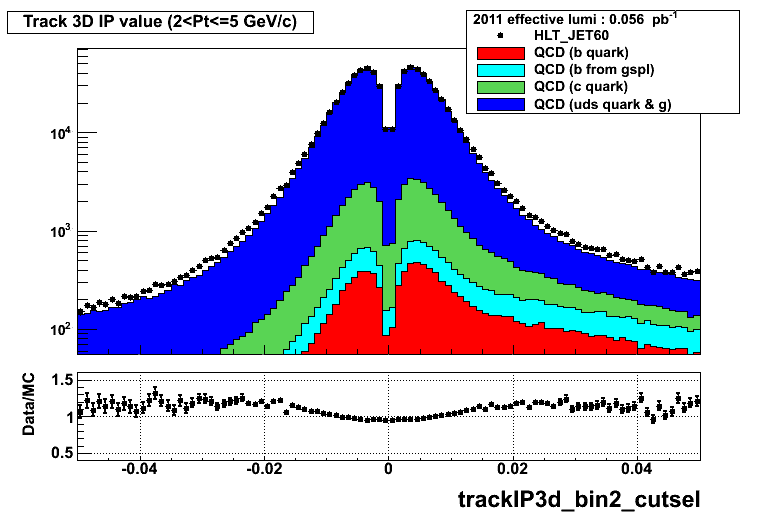
\includegraphics[width=0.32\textwidth]{figures/trackIP3d_bin2_cutsel_Log.png}
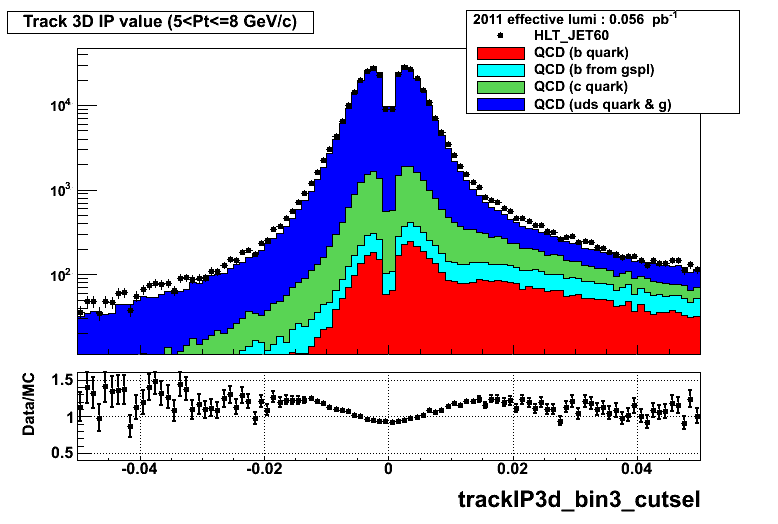
\includegraphics[width=0.32\textwidth]{figures/trackIP3d_bin3_cutsel_Log.png}
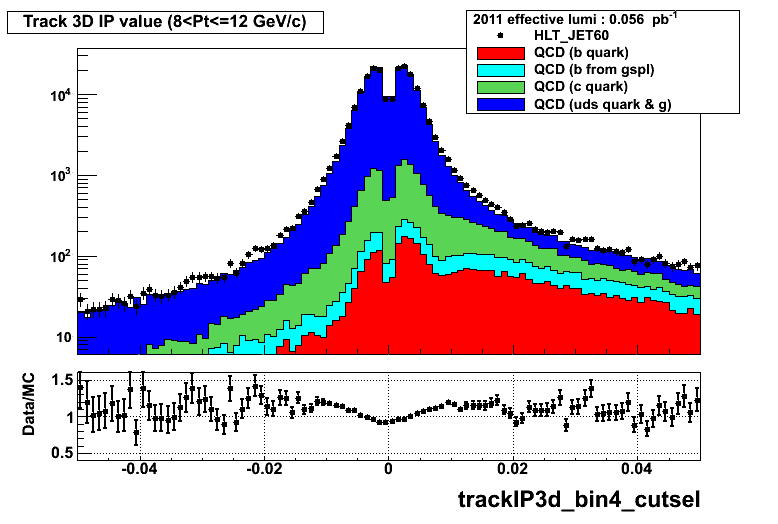
\includegraphics[width=0.32\textwidth]{figures/trackIP3d_bin4_cutsel_Log.png}
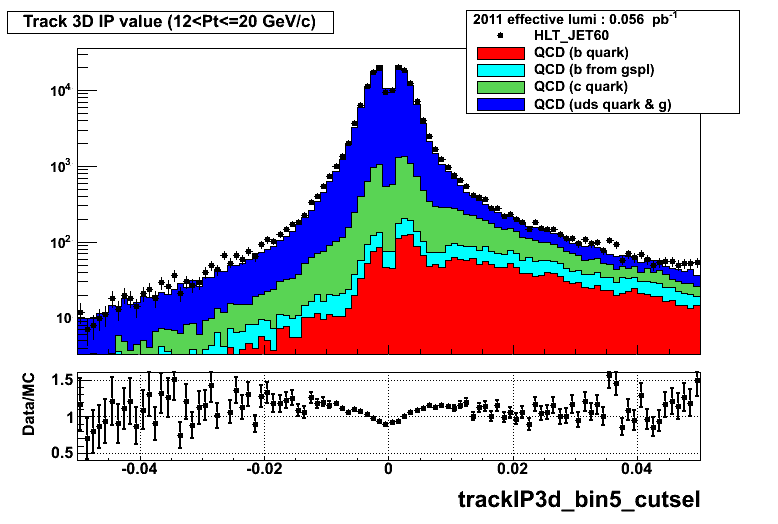
\includegraphics[width=0.32\textwidth]{figures/trackIP3d_bin5_cutsel_Log.png}
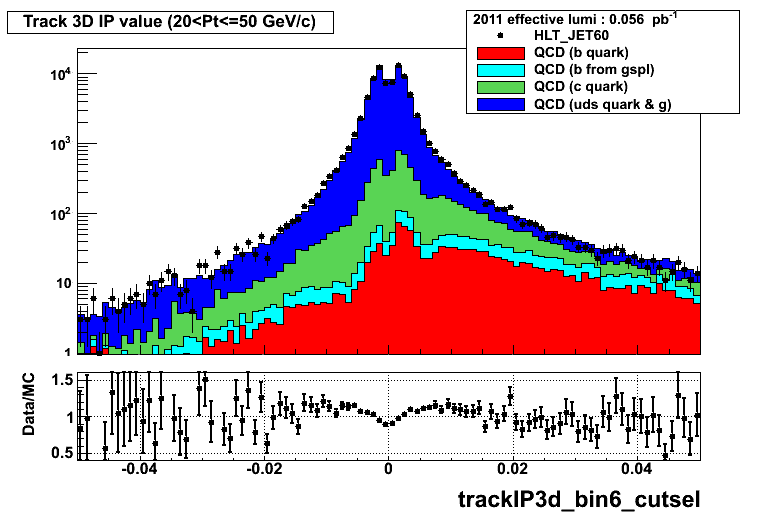
\includegraphics[width=0.32\textwidth]{figures/trackIP3d_bin6_cutsel_Log.png}
\caption{The IP value in six bins of track $p_t$. From top left to bottom right (in units of GeV/$c$): $1<p_t<2; \ 2<p_t<5; \ 5<p_t<8; \ 8<p_t<12; \ 12<p_t<20; \ 20<p_t<50$.   }
\label{fig:IPbinnedTrackpt}
\end{figure}


\clearpage
\section{Secondary vertices \label{sec:secondaryvertex}}
Secondary vertex reconstruction is performed using the “Adaptive Vertex Finder” \cite{bib:AVF}, which performs a fully inclusive vertex search in a list of given tracks. The approach is to fit a vertex from all tracks
and iteratively repeat the fit with tracks that were not compatible with the vertices obtained
in previous iterations. This procedure is repeated until the list of tracks is exhausted or the
vertex fit fails. The “Adaptive Vertex Fitter” is used for the actual vertex fit performed at each
iteration. Since all candidate tracks are passed to it at once, it is able to intrinsically identify and
deal with outliers to allow for the fit to converge. It therefore applies an iterative procedure, by which outlier tracks are increasingly downweighted. This is done until the fit converges and
thus only compatible tracks, which have sizable weights, remain.

The parameters used are primcut = 1.8 and seccut = 6.0. Both denote the track-vertex compatibility
cutoff parameter used for the first and all subsequent fits, respectively. The first fit
attempt is additionally constrained to the beam spot in order to avoid a successful fit of a secondary
vertex with the small cutoff parameter designed for identification of tracks from the
primary vertex. The cutoff parameter of 6.0 is deliberately chosen this large in order to increase
the vertexing efficiency for cases of a b-c decay chain where the two individual secondary and
tertiary vertices cannot be resolved, but both decays yield enough tracks to form a common
vertex. While this vertex definition is slightly unphysical, it increases the b-tagging performance
of the “combined secondary vertex” algorithm. The vertex finder considers a track to
be an outlier if it has been assigned a fit weight of less than 0.5.

The resulting list of vertices is then subject to a cleaning procedure which applies the following
selection criteria:
\begin{itemize}
\item fraction of tracks shared with primary vertex $< 0.65$
\item distance from beam spot in transverse plane $< 2.5$ cm
\item DR of the flight direction with respect to the jet axis $< 0.5$
\item $D_{xy}/\sigma_{D_{xy}}$ (2D “flight distance” significance with respect to reconstructed primary
vertex) $> 3$
\item $D_{xy} > 0.1$ mm
\end{itemize}
In addition, a rejection of vertices due to $K_s$ mesons is applied by rejecting vertices with an invariant mass in the $K_s$ mass window of $0.5 \pm 0.05$~GeV$/c^2$. 


The average charged track multiplicity of a B hadron decay is about five and despite the tight
track quality cuts the efficiency of being able to reconstruct respective decay vertices is very
high. Efficiency limiting factors in reconstruction arise from tracking inefficiencies, tracks lost
due to quality or acceptance cuts or tracks that are also compatible with the primary vertex and
hence excluded from the secondary vertex fit. The number of reconstructed vertices per jet is shown on the left in Figure \ref{fig:vertexNtracks}, while  the number of tracks at the reconstructed secondary vertex is shown in the middle. The dependence of the track multiplicity on the jet momentum is shown on the right. It is visible that the fraction ob b-jets is significantly enhanced for vertices with three or more tracks. This is also visible in  Figure \ref{fig:vertexMass} which shows the reconstructed vertex mass with a minimum of two (left plot) or three (middle plot) tracks at the Secondary Vertex. The right plot in Figure \ref{fig:vertexMass} shows the transverse momentum of the secondary vertex (with two tracks) which is determined using the sum of the momentum vectors of the  tracks at the vertex.

\begin{figure}[h!]
\centering
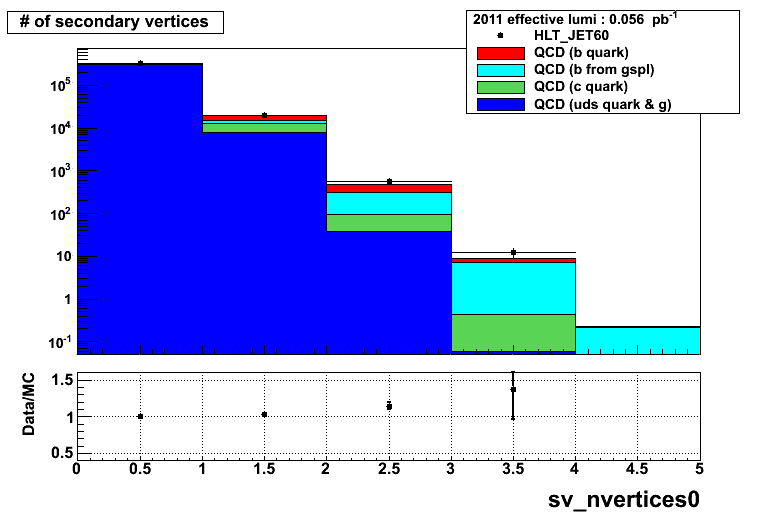
\includegraphics[width=0.32\textwidth]{figures/sv_nvertices0_Log.png}
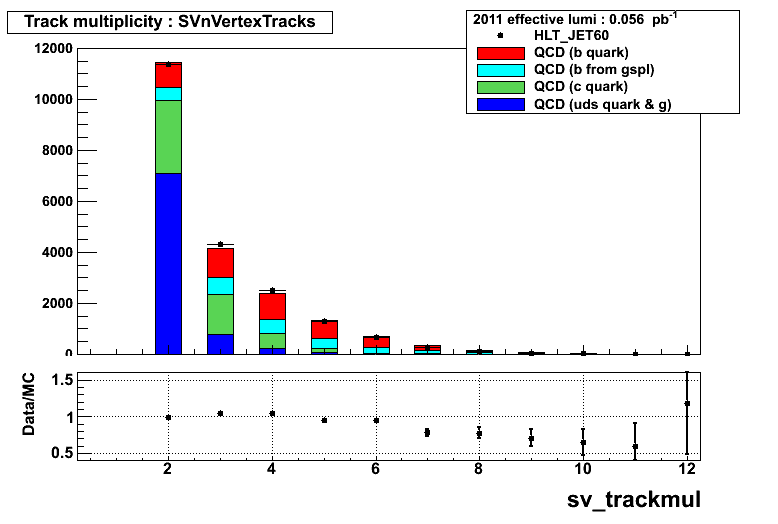
\includegraphics[width=0.32\textwidth]{figures/sv_trackmul_Linear.png}
\includegraphics[width=0.32\textwidth]{figures/sv_track_vs_jetpt_Linear.png}
\caption{Left: number of reconstructed secondary vertices per jet, middle: number of tracks at the reconstructed secondary vertex, right: average number of tracks at the secondary vertex versus jet $p_t$. }
\label{fig:vertexNtracks}
\end{figure}

\begin{figure}[h!]
\centering
\includegraphics[width=0.32\textwidth]{figures/sv_mass_Linear.png}
\includegraphics[width=0.32\textwidth]{figures/sv_mass_3tr_Linear.png}
\includegraphics[width=0.32\textwidth]{figures/sv_vtx_pt_Linear.png}
\caption{Left: vertex mass with two or more reconstructed tracks at the vertex. Middle: vertex mass with three or more tracks at the vertex. Right: transverse momentum of the secondary vertex (with two or more tracks). }
\label{fig:vertexMass}
\end{figure}


An important quantity which is sensitive to the lifetime of B hadron decays is the  distance between primary and secondary vertex. As for the impact paramter, the significance of this quantity is used in b-tagging algorithms. Figure \ref{fig:vertexdistance} shows the flight distance significance, the normalized $\chi^2$ of the vertex fit and the energy ratio of tracks at the secondary vertex with respect to all tracks in the jet.

\begin{figure}[h!]
\centering
\includegraphics[width=0.32\textwidth]{figures/sv_flightsig3d_Log.png}
\includegraphics[width=0.32\textwidth]{figures/sv_eratio_Linear.png}
\includegraphics[width=0.32\textwidth]{figures/sv_normchi2_Linear.png}
\caption{Left: vertex flight distance significance. Middle: ratio of track energy at the secondary vertex with respect to all selected tracks in the jet. Right: vertex fit normalized $\chi^2$. }
\label{fig:vertexdistance}
\end{figure}

Two different directions can be defined at the secondary vertex: the flight direction, which points from the primary vertex to the secondary vertex and the direction of the vertex momentum which is the sum of all vertex track momenta. The angle between these two directions measured in $\Delta R$ as well as the angle with the jet axis are shown in Figure~\ref{fig:vertexAngles}.

\begin{figure}[h!]
\centering
\includegraphics[width=0.32\textwidth]{figures/sv_deltar_jet_Linear.png}
\includegraphics[width=0.32\textwidth]{figures/sv_deltar_sum_jet_Linear.png}
\includegraphics[width=0.32\textwidth]{figures/sv_deltar_sum_dir_Linear.png}
\caption{Left: angular distance in $\Delta R$ between jet axis and vertex direction. Middle: angular distance in $\Delta R$ between jet axis and the sum of track momenta at the vertex, Right: angular distance in $\Delta R$ between vertex direction and the sum of track momenta at the vertex. }
\label{fig:vertexAngles}
\end{figure}
\clearpage
\section{Discriminators and tagging rates \label{sec:discriminators}}
Details about the calculation of the discriminators are given in~\cite{btaggingPAS2009}. The distributions of track counting discriminators are shown in Figure~\ref{fig:trackCountingDisc}, jet probability discriminators are shown in Figure~\ref{fig:JetProbDisc} and simple secondary vertex discriminators are shown in Figure~\ref{fig:SimpleSVDisc}. 

\begin{figure}[h!]
\centering
\includegraphics[width=0.45\textwidth]{figures/discri_tche_Log.png}
\includegraphics[width=0.45\textwidth]{figures/discri_tchp_Log.png}
\caption{Left: track counting high efficiency, Right: track counting high purity discriminators. }
\label{fig:trackCountingDisc}
\end{figure}
\begin{figure}[h!]
\centering
\includegraphics[width=0.45\textwidth]{figures/discri_jetprob_Log.png}
\includegraphics[width=0.45\textwidth]{figures/discri_jetbprob_Log.png}
\caption{Left: jet probability , Right: jet B probability discriminators. }
\label{fig:JetProbDisc}
\end{figure}
\begin{figure}[h!]
\centering
\includegraphics[width=0.45\textwidth]{figures/discri_ssche_Linear.png}
\includegraphics[width=0.45\textwidth]{figures/discri_sschp_Linear.png}
\caption{Left: simple secondary vertex high efficiency , Right: simple secondary vertex high purity discriminators. The underflow bin for jets which do not contain a reconstructed secondary vertex is not displayed.}
\label{fig:SimpleSVDisc}
\end{figure}

The tagging rates can be calculated by integrating the discriminator distributions (Figures \ref{fig:trackCountingDisc} to \ref{fig:SimpleSVDisc}) from a given discriminator cut to infinity, divided by the total integral.  The tagging rates are displayed in Figures~\ref{fig:trackCountingDiscEff} to \ref{fig:SimpleSVDiscEff}.

\begin{figure}[h!]
\centering
\includegraphics[width=0.45\textwidth]{figures/tagRate_discri_tche_Log.png}
\includegraphics[width=0.45\textwidth]{figures/tagRate_discri_tchp_Log.png}
\caption{Left: track counting high efficiency tagging rate, Right: track counting high purity tagging rate. }
\label{fig:trackCountingDiscEff}
\end{figure}
\begin{figure}[h!]
\centering
\includegraphics[width=0.45\textwidth]{figures/tagRate_discri_jetprob_Log.png}
\includegraphics[width=0.45\textwidth]{figures/tagRate_discri_jetbprob_Log.png}
\caption{Left: jet probability tagging rate, Right: jet B probability tagging rate. }
\label{fig:JetProbDiscEff}
\end{figure}
\begin{figure}[h!]
\centering
\includegraphics[width=0.45\textwidth]{figures/tagRate_discri_ssche_Linear.png}
\includegraphics[width=0.45\textwidth]{figures/tagRate_discri_sschp_Linear.png}
\caption{Left: simple secondary vertex high efficiency tagging rate, Right: simple secondary vertex high purity tagging rate. }
\label{fig:SimpleSVDiscEff}
\end{figure}
\clearpage
\section{Muons in jets \label{sec:muonjets}}
This section describes the special properties of jets containing muons. As mentioned in Section \ref{sec:samples}, a dedicated di-jet plus muon trigger has been used in data. The Monte Carlo samples are similar to the QCD samples used in the previous section except for the requirement of the presence of a muon at generator level.


Muons are
seeded from the CMS muon chambers, and are then linked to tracks found
in the tracking system to form global muons
\cite{JINST,CMS_PAS_MUO-10-002}.

The muon selection requirements are the following:
\begin{itemize}
\item transverse momentum $p_t >$ 7 GeV 
\item number of valid inner hits $>$ 10
\item number of pixel hits $>$ 1
\item number of missed outer hits $<$ 3
\item number of matches $>$ 0
\item inner $\chi^2 / ndof <$ 10
\item global  $\chi^2 / ndof <$ 10
\item longitudinal distance to primary vertex $<$ 2 cm
\item $\Delta$R to jet axis $<$ 0.4
\end{itemize}

Figure \ref{fig:muonplots1} shows the transverse momentum,  the impact parameter significance and the reconstructed number of muons per jet.


\begin{figure}[h!]
\centering
\includegraphics[width=0.32\textwidth]{figures/mujetmuon_Pt_Log.png}
\includegraphics[width=0.32\textwidth]{figures/mujetmuons_multiplicity_Log.png}
\includegraphics[width=0.32\textwidth]{figures/mujetmuon_Sip3d_Log.png}
\caption{Left: transverse momentum $p_t$ of muons in jets. Middle: number of reconstructed muons per jet. Right: 3D impact parameter significance of muons in jets.}
\label{fig:muonplots1}
\end{figure}



An important quantity for performance measurements is the relative transverse momentum with respect to the jet, $p_t^{rel}$. This is displayed in Figure \ref{fig:muonplots2} (left). There is an apparent discrepancy in this distribution which is also visible in the angle between the muon and the jet axis in units of $\Delta$R (Figure \ref{fig:muonplots2} right).

\begin{figure}[h!]
\centering
\includegraphics[width=0.42\textwidth]{figures/mujetmuon_ptrel_Linear.png}
\includegraphics[width=0.42\textwidth]{figures/mujetmuon_DeltaR_Linear.png}
\caption{Left: transverse momentum of the muon with respect to the jet axis $p_t^{rel}$. Right: angle (in units of $\Delta R$) between the muon and the jet axis.}
\label{fig:muonplots2}
\end{figure}

The angular discrepancies in muon-jets are also visible in the secondary vertex angles. Figure \ref{fig:vertexAnglesMuJets}  shows the same distributions as Figure \ref{fig:vertexAngles}, but for jets with muons. The trend towards larger angles in data is enhanced in muon jets.

\begin{figure}[h!]
\centering
\includegraphics[width=0.32\textwidth]{figures/mujetsv_deltar_jet_Linear.png}
\includegraphics[width=0.32\textwidth]{figures/mujetsv_deltar_sum_jet_Linear.png}
\includegraphics[width=0.32\textwidth]{figures/mujetsv_deltar_sum_dir_Linear.png}
\caption{Left: angular distance in $\Delta R$ between jet axis and vertex direction. Middle: angular distance in $\Delta R$ between jet axis and the sum of track momenta at the vertex, Right: angular distance in $\Delta R$ between vertex direction and the sum of track momenta at the vertex. }
\label{fig:vertexAnglesMuJets}
\end{figure}
\cleardoublepage
\section{Alignment \label{sec:alignment}}

%%%%%%%%%%%%%%%%%%%%%%%%%%%%%%%%%%%%%%%%%%%%%%%%%%%%%%%%%%%%%%%%%%%%
\subsection{Alignment of the Inner Silicon Tracker}
%%%%%%%%%%%%%%%%%%%%%%%%%%%%%%%%%%%%%%%%%%%%%%%%%%%%%%%%%%%%%%%%%%%%
The determination of the alignment corrections for the Inner Silicon
Tracker to be used for the reprocessing of the 2010 data was done with
the global method~\cite{TkAl_VBlobel,TkAl_Millepede} using a mixture of tracks coming
from atmospheric cosmic rays and minimum bias collisions. 
The global method aligns the highest level structures (half-barrels, endcaps) with all
the six degrees of freedom together with all module units with the most sensitive 
degrees of freedom each: $u$, $w$ and $\gamma$ for the strip modules (also $\alpha$ and $\beta$ in TIB)
and $u$, $v$, $w$ and $\gamma$ for the pixel modules~\footnote{
A local right-handed coordinate system is defined for each module, with $u$ being the
more precisley measured coordinate, $v$ orhogonal to the $u$-axis and in the 
module plane, and the $w$-axis normal to the module plane. Angles $\alpha$, $\beta$ and $\gamma$ are the rotations
around the $u$, $v$ and $w$-axes respectively.}.

During the 2010 LHC run, the geometry of the pixels was monitored on a
daily basis  using the so-called unbiased track-to-primary vertex
residuals. This method consists in selectively
removing a track from the event, determine a primary vertex with the
others, compute the transverse and longitudinal projections of impact
parameter of the probe track with respect the primary vertex and
finally studying the mean value of the distribution of the residuals
as a function of $\phi$, $\eta$ of the track.

Despite starting from a pre-calibrated detector, a discontinuity in
the distribution of the mean longitudinal impact parameter as a
function of azimuthal angle was observed, with the height of the step changing
few times during the year. 
This behavior was interpreted as relative movements, up to 90 $\mu$m in
magnitude, along the $z$-direction of the two BPIX half-barrels,
movements which are allowed since the two halves are mechanically independent.

To cope with this, in a common fit separate sets of alignment corrections for each of
the three BPIX layers in each half-barrel and each of the four FPIX
half-disks in each endcap were provided for seven different periods of
the data-taking. The relative position of the modules with
respect the supporting structure was instead assumed to be the same along all
the 2010 data-taking. 
Figure~\ref{fig:TkAl_PV} shows the distribution of longitudinal separation of the BPIX 
half-barrels as estimated from the unbiased track-to-primary vertex residuals 
as a function of time before and after the alignment procedure. 
 
The statistical precision reached by the alignment was checked looking at the
distribution of the median of the unbiased track-to-hit residuals
computed for each module. 
%In the pixel subsystem, the most relevant component for b-tagging, 
The RMS of these distributions amount to 2 $\mu$m (4 $\mu$m) for the r-$\phi$ ($z$) measurement
coordinate in the BPIX and to 6 $\mu$m (11 $\mu$m) for the r-$\phi$
($r$) measurement in the FPIX, for all the data-taking intervals described above.

A set of alignment parameter errors, calibrated to provide pulls of
the track-to-hit residuals with gaussian standard deviation close to
unity, was provided together with the alignment
constants.

Finally, prior to the restart of the 2011 LHC operations, the alignment
corrections for the two BPIX half-barrels (6 dofs) and for the four FPIX half-disks
(3 translational dofs) were recomputed using a sample of about 15k cosmic ray
tracks.
The analysis of the track-to-primary vertex residuals on events from
2011 collisions indicates that a potentially uncorrected separation of
the two BPIX half-barrels is at most 10 $\mu$m.


%%%%%%%%%%%%%%%%%%%%%%%%%%%%%%%%%%%%%%%%%%%%%%%%%%%%%%%%%%%%%%%%%%%%
\subsection{Simulation-based study of the impact of misalignment on
  b-tagging performances}
%%%%%%%%%%%%%%%%%%%%%%%%%%%%%%%%%%%%%%%%%%%%%%%%%%%%%%%%%%%%%%%%%%%%

The performance of the alignment procedure described above is
essentially not limited by the statistical precision.
To properly describe in the simulation the alignment
accuracy reached at the end of 2010, a misalignment scenario was
prepared following the same approach described in ~\cite{TkAl_CRAFT08}
and using a sample of simulated events with approximately the
same composition of the sample used for the alignment in the data. 
The same alignment parameter errors determined in the data
complemented the misalignment scenario, hereafter referred to as MC2010.

The performances of the different b-tagging algorithms obtained with
the MC2010 misalignment scenario were compared with respect those
obtained with a perfectly aligned detector and with a misalignment
scenario, prepared before the installation of the Inner Silicon Tracker
in CMS, supposed at that epoch to describe the uncertainty on the
alignment parameters expected after 10/pb of collected data~\cite{CMS_NOTE_2008-29}.
The results, obtained from a sample of about 1.5 millions simulated
$t\bar{t}$ events are shown in Figure~\ref{fig:TkAl_effpur_newstartup_vs_ideal}.
For all the taggers the performance with the MC2010 scenario are equal
to those obtained with a perfectly aligned detector.

The same sample of simulated events was used to evaluate the deterioration of the
performances of the b-tagging algorithms in case shifts along the
$z$-direction of the two BPIX half-barrels, similar to those observed
in 2010, were present but not corrected by the alignment procedure.
For this study, the positions and orientations of all the other components of the Tracker 
were supposed to be perfectly known.

Three different scenarios  were investigated
corresponding to 40 $\mu$m, 80 $\mu$m and 160 $\mu$m absolute separation of the
BPIX half-barrels. 
No change in the b-tagging performance is observed for the SSVHE
and SSVHP taggers. For the other taggers
(Figure~\ref{fig:TkAl_effpur_zshifts_vs_ideal}), a significant decrease
of the b-tagging efficiency  is observed only for the 160 $\mu$m separation.
For the track-counting taggers the decrease is more pronounced for 
TCHP, about -5.5\% decrease, already setting-in at the medium
contamination working point, while for the TCHE the decrease is visible
only at the loose contamination working point (about -2.5\% reduction).
In case of the CSVB tagger the decrease is about -2.5\% at 160 $\mu$m separation. 
The largest drop in b-tagging efficiency is observed for the JP and JBP taggers, about -7\%   
at all the tight, medium and loose working points
for the 160 $\mu$m separation scenario.

 

\begin{figure}[!h]
  \centering
    \includegraphics[width=0.7\textwidth]{figures/TkAl_PV}
    \caption{Longitudinal separation of the BPIX half-barrels as
      estimated from the unbiased track-to-primary vertex residual
      method as a function of time for the 2010 LHC proton-proton
      run. Empty (filled) dots are the pre-(post-)alignment values.}
    \label{fig:TkAl_PV}
\end{figure}

\begin{figure}[!h]
  \centering
    \includegraphics[width=0.45\linewidth]{figures/TkAl_MC2010_TCHE}
    \includegraphics[width=0.45\linewidth]{figures/TkAl_MC2010_TCHP}
    \includegraphics[width=0.45\linewidth]{figures/TkAl_MC2010_CSV}
    \includegraphics[width=0.45\linewidth]{figures/TkAl_MC2010_JP}
    \caption{Contamination vs. efficiency for the TCHE, TCHP, CSV and JP b-tagging
      algorithms for a scenario describing the estimated current
      accuracy in alignment compared to a perfectly aligned detector.
      For reference the performance expected 
    after 10/pb of collected lumi, based on a previuos study, are also shown.}
    \label{fig:TkAl_effpur_newstartup_vs_ideal}
\end{figure}

\begin{figure}[!h]
  \centering
    \includegraphics[width=0.45\linewidth]{figures/TkAl_BPIXHBDZ_TCHE}
    \includegraphics[width=0.45\linewidth]{figures/TkAl_BPIXHBDZ_TCHP}
    \includegraphics[width=0.45\linewidth]{figures/TkAl_BPIXHBDZ_CSV}
    \includegraphics[width=0.45\linewidth]{figures/TkAl_BPIXHBDZ_JP}
    \caption{Contamination vs. efficiency for the TCHE, TCHP, CSV and JP b-tagging
      algorithms for scenarios with an artificial separation of the two BPIX
      half-barrels of 40, 80, 160 $\mu$m.}
    \label{fig:TkAl_effpur_zshifts_vs_ideal}
\end{figure}


\clearpage
\section{Pileup \label{sec:pileup}}
Due to the high LHC luminosity in the 2011, several proton collisions are taking place simultaneously in one bunch crossing. The number of reconstructed primary vertices per event is shown in Figure \ref{fig:Npv}. The constant change of the luminosity conditions makes a correct simulation in the Monte Carlo samples difficult. We therefore use Figure \ref{fig:Npv} to obtain reweighting factors to equalize the vertex multiplicity in Monte Carlo. The reweighting procedure has been applied for the results shown in Section \ref{sec:impactparameter} to \ref{sec:muonjets}.

\begin{figure}[h!]
\centering
\includegraphics[width=0.49\textwidth]{figures/npv_no_scaled_Linear.png}
\caption{Number of reconstructed primary vertices per event.}
\label{fig:Npv}
\end{figure}

The signal primary vertex is chosen to be the one with the largest sum of track $p_t^2$ which is currently the standard CMS convention. Tracks from pileup vertices can be wrongly associated to a jet from the signal vertex. This effect is visible in Figure \ref{fig:pvNTracks} (left) which shows the number of tracks associated to a jet for three different primary vertex multiplicities. The right plot in Figure \ref{fig:pvNTracks} shows the number of selected tracks. The track selection is clearly rejecting those additional tracks from nearby primary vertices. The most efficient observable to  reject pileup tracks is the distance of the track to the jet axis (compare Section \ref{sec:trackselection}). In the ideal case, tracks from B decays are tangential to the jet axis and therefore have zero distance to the jet axis. Tracks  from pileup events are well separated from the jet axis in longitudinal direction.

\begin{figure}[h!]
\centering
\includegraphics[width=0.42\textwidth]{figures/npv_ntracks_jet_Linear.png}
\includegraphics[width=0.42\textwidth]{figures/npv_ncutseltracks_jet_Linear.png}
\caption{Left: number of tracks associated to a jet without any selection cuts. Right: number of tracks associated to a jet passing the selection cuts.}
\label{fig:pvNTracks}
\end{figure}

Some additional validation plots, for three different vertex multiplicities are shown in Figure \ref{fig:pvSVobservables}. The most important observables, such as impact parameter and vertex flight distance seem to be in good agreement among the different pileup multiplicities.  The number of reconstructed secondary vertices per jet for the three pileup cases is shown in Figure \ref{fig:pvSVmult}.




\begin{figure}[h!]
\centering
\includegraphics[width=0.32\textwidth]{figures/npv_IP3d2sig0_Log.png}
\includegraphics[width=0.32\textwidth]{figures/npv_flightsig3d_Log.png}
\includegraphics[width=0.32\textwidth]{figures/npv_svmass_Linear.png}
\caption{Left: impact parameter significance of the second track, ordered by IP significance. Middle: secondary vertex flight distance significance. Right: secondary vertex mass. All distributions are split into three different primary vertex multiplicities.}
\label{fig:pvSVobservables}
\end{figure}

\begin{figure}[h!]
\centering
\includegraphics[width=0.42\textwidth]{figures/npv_nsv0_Log.png}
\includegraphics[width=0.42\textwidth]{figures/npv_nsv0_3tr_Log.png}
\caption{Left (right): number of reconstructed secondary vertices with three (two) tracks per jet. The distributions are split into three different primary vertex multiplicities.}
\label{fig:pvSVmult}
\end{figure}


However, Figure \ref{fig:pvNTracks} (right) indicates a slightly reduced track selection efficiency for high pileup multiplicities, because the average number of tracks decreases with more pileup. This results in a reduced b-tagging efficiency in pileup events.
A Monte Carlo based study has been done which shows a clear degradation of the b-tagging performance for events with pileup. This is illustrated in Figure \ref{fig:pileupBTagPerformance} which shows the light flavor mistag efficiency versus b-tagging efficiency for several b-tagging algorithms.

\begin{figure}[h!]
\centering
\includegraphics[width=0.32\textwidth]{figures/pileupPerfTCHE.png}
\includegraphics[width=0.32\textwidth]{figures/pileupPerfTCHP.png}
\includegraphics[width=0.32\textwidth]{figures/pileupPerfSSV.png}
\caption{Light flavor mistag efficiency versus b-tagging efficiency for different piluep scenarios. ({\bf FIXME: produce plots properly}). Left: track counting high efficiency algorithm. Middle: track counting high purity algorithm. Right: simple secondary vertex high efficiency algorithm. }
\label{fig:pileupBTagPerformance}
\end{figure}


({\bf FIXME:})    discussion on PV-jet association
\section{Development of new algorithms \label{sec:dvelopments}}

\subsection{Improved jet-track association}

\subsection{Combined secondary vertex algorithm}

The discrimination power of all secondary vertex $b$-taggers described
in \cite{btaggingPAS2009} can be further improved by combining them in
a multivariate analysis (MVA) \cite{Weiser:2006md}.  A new
implementation of this technique is in development, using a general
MVA framework in CMSSW.

A simple classifier was chosen as a first step, to make sure that the
workflow is well-understood.  Input variables are combined using a Naive
Bayes likelihood ratio (which assumes that they are uncorrelated), and
are normalized and rotated to remove linear correlations.

The discriminator is separately optimized in three broad classes: RecoVertex (a
secondary vertex is fully reconstructed), PseudoVertex (no secondary
vertex is reconstructed, but at least two tracks are inconsistent with
the primary vertex with a transverse impact parameter significance
greater than 2.0), and NoVertex (neither of the above).  These classes
determine the set of input variables available for optimization.

The work on this project is ongoing.  The MVA framework is modular
enough to replace classification engines with minimal impact on the
workflow; thus, the project has a natural upgrade path to more
sophisticated MVA techniques.

%
%% **DO NOT REMOVE BIBLIOGRAPHY**
\bibliography{auto_generated}   % will be created by the tdr script.

%% examples of appendices. **DO NOT PUT \end{document} at the end
\clearpage
\appendix
\section{Appendix \label{sec:AppendixA}}
Figures \ref{fig:HLTJet30IPfirstTrack} to \ref{fig:HLTJet30vertexAnglesMuJets} show a selection of the plots from Sections \ref{sec:impactparameter} to \ref{sec:muonjets} but with a lower trigger threshold  (\verb|HLT_Jet30| in data and \verb|HLTJet15U| in Monte Carlo)  and lower jet momentum cut of $p_t >$ 30 GeV in case of the single jet triggers.  For the b-jet triggers another set of plots has been produced with \verb|HLT_BTagMu_DiJet20_Mu5|, requiring two jets with $p_t >$ 40 GeV, one of them with $p_t >$ 45 GeV.

\begin{figure}[h!]
\centering
\includegraphics[width=0.32\textwidth]{figures/HLTJet30IP3d1sorted_Log.png}
\includegraphics[width=0.32\textwidth]{figures/placeholder.png}
\includegraphics[width=0.32\textwidth]{figures/HLTJet30IP3d1sigsorted_Log.png}
\caption{Left: IP value, middle: IP error, right: IP significance for the first track in the jet, ordered by IP significance.  }
\label{fig:HLTJet30IPfirstTrack}
\end{figure}

\begin{figure}[h!]
\centering
\includegraphics[width=0.32\textwidth]{figures/HLTJet30IP3d2sorted_Log.png}
\includegraphics[width=0.32\textwidth]{figures/placeholder.png}
\includegraphics[width=0.32\textwidth]{figures/HLTJet30IP3d2sigsorted_Log.png}
\caption{Left: IP value, middle: IP error, right: IP significance for the second track in the jet, ordered by IP significance.  }
\label{fig:HLTJet30IPsecondTrack}
\end{figure}

\begin{figure}[h!]
\centering
\includegraphics[width=0.32\textwidth]{figures/HLTJet30IP3d3sorted_Log.png}
\includegraphics[width=0.32\textwidth]{figures/placeholder.png}
\includegraphics[width=0.32\textwidth]{figures/HLTJet30IP3d3sigsorted_Log.png}
\caption{Left: IP value, middle: IP error, right: IP significance for the third track in the jet, ordered by IP significance.  }
\label{fig:HLTJet30IPThirdTrack}
\end{figure}

\begin{figure}[h!]
\centering
\includegraphics[width=0.32\textwidth]{figures/HLTJet30trackIP3d_cutsel_Log.png}
\includegraphics[width=0.32\textwidth]{figures/HLTJet30trackIP3dError_cutsel_Log.png}
\includegraphics[width=0.32\textwidth]{figures/HLTJet30trackIP3dsig_cutsel_Log.png}
\caption{Left: IP value, middle: IP error, right: IP significance for all selected tracks in the jet. The track selection as defined in Section~\ref{sec:trackselection} has been applied.}
\label{fig:HLTJet30IPAllTrack}
\end{figure}

\begin{figure}[h!]
\centering
\includegraphics[width=0.32\textwidth]{figures/HLTJet30sv_nvertices0_Log.png}
\includegraphics[width=0.32\textwidth]{figures/HLTJet30sv_trackmul_Linear.png}
\includegraphics[width=0.32\textwidth]{figures/placeholder.png}
\caption{Left: number of reconstructed secondary vertices per jet, middle: number of tracks at the reconstructed secondary vertex, right: average number of tracks at the secondary vertex versus jet $p_t$. }
\label{fig:HLTJet30vertexNtracks}
\end{figure}

\begin{figure}[h!]
\centering
\includegraphics[width=0.32\textwidth]{figures/HLTJet30sv_mass_Linear.png}
\includegraphics[width=0.32\textwidth]{figures/HLTJet30sv_mass_3tr_Linear.png}
\includegraphics[width=0.32\textwidth]{figures/HLTJet30sv_vtx_pt_Linear.png}
\caption{Left: vertex mass with two or more reconstructed tracks at the vertex. Middle: vertex mass with three or more tracks at the vertex. Right: transverse momentum of the secondary vertex (with two or more tracks). }
\label{fig:HLTJet30vertexMass}
\end{figure}

\begin{figure}[h!]
\centering
\includegraphics[width=0.32\textwidth]{figures/HLTJet30sv_flightsig3d_Log.png}
\includegraphics[width=0.32\textwidth]{figures/HLTJet30sv_eratio_Linear.png}
\includegraphics[width=0.32\textwidth]{figures/HLTJet30sv_normchi2_Linear.png}
\caption{Left: vertex flight distance significance. Middle: ratio of track energy at the secondary vertex with respect to all selected tracks in the jet. Right: vertex fit normalized $\chi^2$. }
\label{fig:HLTJet30vertexdistance}
\end{figure}

\begin{figure}[h!]
\centering
\includegraphics[width=0.32\textwidth]{figures/HLTJet30sv_deltar_jet_Linear.png}
\includegraphics[width=0.32\textwidth]{figures/HLTJet30sv_deltar_sum_jet_Linear.png}
\includegraphics[width=0.32\textwidth]{figures/HLTJet30sv_deltar_sum_dir_Linear.png}
\caption{Left: angular distance in $\Delta R$ between jet axis and vertex direction. Middle: angular distance in $\Delta R$ between jet axis and the sum of track momenta at the vertex, Right: angular distance in $\Delta R$ between vertex direction and the sum of track momenta at the vertex. }
\label{fig:HLTJet30vertexAngles}
\end{figure}

\begin{figure}[h!]
\centering
\includegraphics[width=0.45\textwidth]{figures/HLTJet30discri_tche_Log.png}
\includegraphics[width=0.45\textwidth]{figures/HLTJet30discri_tchp_Log.png}
\caption{Left: track counting high efficiency, Right: track counting high purity discriminators. }
\label{fig:HLTJet30trackCountingDisc}
\end{figure}
\begin{figure}[h!]
\centering
\includegraphics[width=0.45\textwidth]{figures/HLTJet30discri_jetprob_Log.png}
\includegraphics[width=0.45\textwidth]{figures/HLTJet30discri_jetbprob_Log.png}
\caption{Left: jet probability , Right: jet B probability discriminators. }
\label{fig:HLTJet30JetProbDisc}
\end{figure}
\begin{figure}[h!]
\centering
\includegraphics[width=0.45\textwidth]{figures/HLTJet30discri_ssche_Linear.png}
\includegraphics[width=0.45\textwidth]{figures/HLTJet30discri_sschp_Linear.png}
\caption{Left: simple secondary vertex high efficiency , Right: simple secondary vertex high purity discriminators. The underflow bin for jets which do not contain a reconstructed secondary vertex is not displayed.}
\label{fig:HLTJet30SimpleSVDisc}
\end{figure}

\begin{figure}[h!]
\centering
\includegraphics[width=0.45\textwidth]{figures/placeholder.png}
\includegraphics[width=0.45\textwidth]{figures/placeholder.png}
\caption{Left: track counting high efficiency tagging rate, Right: track counting high purity tagging rate. }
\label{fig:HLTJet30trackCountingDiscEff}
\end{figure}
\begin{figure}[h!]
\centering
\includegraphics[width=0.45\textwidth]{figures/placeholder.png}
\includegraphics[width=0.45\textwidth]{figures/placeholder.png}
\caption{Left: jet probability tagging rate, Right: jet B probability tagging rate. }
\label{fig:HLTJet30JetProbDiscEff}
\end{figure}
\begin{figure}[h!]
\centering
\includegraphics[width=0.45\textwidth]{figures/placeholder.png}
\includegraphics[width=0.45\textwidth]{figures/placeholder.png}
\caption{Left: simple secondary vertex high efficiency tagging rate, Right: simple secondary vertex high purity tagging rate. }
\label{fig:HLTJet30SimpleSVDiscEff}
\end{figure}

\begin{figure}[h!]
\centering
\includegraphics[width=0.32\textwidth]{figures/HLTbtagmu_dijet20mu5mujetmuonPt_Linear.png}
\includegraphics[width=0.32\textwidth]{figures/placeholder.png}
\includegraphics[width=0.32\textwidth]{figures/placeholder.png}
\caption{Left: transverse momentum $p_t$ of muons in jets. Middle: number of reconstructed muons per jet. Right: 3D impact parameter significance of muons in jets.}
\label{fig:HLTJet30muonplots1}
\end{figure}


\begin{figure}[h!]
\centering
\includegraphics[width=0.42\textwidth]{figures/HLTbtagmu_dijet20mu5mujetmuon_ptrel_Linear.png}
\includegraphics[width=0.42\textwidth]{figures/HLTbtagmu_dijet20mu5mujetmuonDeltaR_Linear.png}
\caption{Left: transverse momentum of the muon with respect to the jet axis $p_t^{rel}$. Right: angle (in units of $\Delta R$) between the muon and the jet axis.}
\label{fig:HLTJet30muonplots2}
\end{figure}

\begin{figure}[h!]
\centering
\includegraphics[width=0.32\textwidth]{figures/HLTbtagmu_dijet20mu5mujetsv_deltar_jet_Linear.png}
\includegraphics[width=0.32\textwidth]{figures/HLTbtagmu_dijet20mu5mujetsv_deltar_sum_jet_Linear.png}
\includegraphics[width=0.32\textwidth]{figures/HLTbtagmu_dijet20mu5mujetsv_deltar_sum_dir_Linear.png}
\caption{Left: angular distance in $\Delta R$ between jet axis and vertex direction. Middle: angular distance in $\Delta R$ between jet axis and the sum of track momenta at the vertex, Right: angular distance in $\Delta R$ between vertex direction and the sum of track momenta at the vertex. }
\label{fig:HLTJet30vertexAnglesMuJets}
\end{figure}

